\documentclass[12pt]{article}
 
\usepackage[margin=1in]{geometry}
\usepackage{amsmath,amsthm,amssymb}
\usepackage{mathtools}
\DeclarePairedDelimiter{\ceil}{\lceil}{\rceil}
%\usepackage{mathptmx}
\usepackage{accents}
\usepackage{comment}
\usepackage{graphicx}
\usepackage{IEEEtrantools}
 \usepackage{float}
 
\newcommand{\N}{\mathbb{N}}
\newcommand{\Z}{\mathbb{Z}}
\newcommand{\R}{\mathbb{R}}
\newcommand{\Q}{\mathbb{Q}}
\newcommand*\conj[1]{\bar{#1}}
\newcommand*\mean[1]{\bar{#1}}
\newcommand\widebar[1]{\mathop{\overline{#1}}}


\newcommand{\cc}{{\mathbb C}}
\newcommand{\rr}{{\mathbb R}}
\newcommand{\qq}{{\mathbb Q}}
\newcommand{\nn}{\mathbb N}
\newcommand{\zz}{\mathbb Z}
\newcommand{\aaa}{{\mathcal A}}
\newcommand{\bbb}{{\mathcal B}}
\newcommand{\rrr}{{\mathcal R}}
\newcommand{\fff}{{\mathcal F}}
\newcommand{\ppp}{{\mathcal P}}
\newcommand{\eps}{\varepsilon}
\newcommand{\vv}{{\mathbf v}}
\newcommand{\ww}{{\mathbf w}}
\newcommand{\xx}{{\mathbf x}}
\newcommand{\ds}{\displaystyle}
\newcommand{\Om}{\Omega}
\newcommand{\dd}{\mathop{}\,\mathrm{d}}
\newcommand{\ud}{\, \mathrm{d}}
\newcommand{\seq}[1]{\left\{#1\right\}_{n=1}^\infty}
\newcommand{\isp}[1]{\quad\text{#1}\quad}

\DeclareMathOperator{\imag}{Im}
\DeclareMathOperator{\re}{Re}
\DeclareMathOperator{\diam}{diam}
\DeclareMathOperator{\Tr}{Tr}
\DeclareMathOperator{\cis}{cis}

\def\upint{\mathchoice%
    {\mkern13mu\overline{\vphantom{\intop}\mkern7mu}\mkern-20mu}%
    {\mkern7mu\overline{\vphantom{\intop}\mkern7mu}\mkern-14mu}%
    {\mkern7mu\overline{\vphantom{\intop}\mkern7mu}\mkern-14mu}%
    {\mkern7mu\overline{\vphantom{\intop}\mkern7mu}\mkern-14mu}%
  \int}
\def\lowint{\mkern3mu\underline{\vphantom{\intop}\mkern7mu}\mkern-10mu\int}




\newenvironment{theorem}[2][Theorem]{\begin{trivlist}
\item[\hskip \labelsep {\bfseries #1}\hskip \labelsep {\bfseries #2.}]}{\end{trivlist}}
\newenvironment{lemma}[2][Lemma]{\begin{trivlist}
\item[\hskip \labelsep {\bfseries #1}\hskip \labelsep {\bfseries #2.}]}{\end{trivlist}}
\newenvironment{exercise}[2][Exercise]{\begin{trivlist}
\item[\hskip \labelsep {\bfseries #1}\hskip \labelsep {\bfseries #2.}]}{\end{trivlist}}
\newenvironment{problem}[2][Problem]{\begin{trivlist}
\item[\hskip \labelsep {\bfseries #1}\hskip \labelsep {\bfseries #2.}]}{\end{trivlist}}
\newenvironment{question}[2][Question]{\begin{trivlist}
\item[\hskip \labelsep {\bfseries #1}\hskip \labelsep {\bfseries #2.}]}{\end{trivlist}}
\newenvironment{corollary}[2][Corollary]{\begin{trivlist}
\item[\hskip \labelsep {\bfseries #1}\hskip \labelsep {\bfseries #2.}]}{\end{trivlist}}

\newenvironment{solution}{\begin{proof}[Solution]}{\end{proof}}
 
\begin{document}
 
% --------------------------------------------------------------
%                         Start here
% --------------------------------------------------------------
\title{Math 122A Homework 4}
\author{Ethan Martirosyan}
\date{\today}
\maketitle
\hbadness=99999
\hfuzz=50pt
\section*{Chapter 2 Problem 2}
In order for $(z-a)/(z-b)$ to be on the unit circle, we must have $\vert (z-a)/(z-b) \vert = 1$. Since $z$ is assumed to be on the perpendicular bisector of $a$ and $b$, it must be equidistant from $a$ and $b$; that is, $\vert z - a \vert = \vert z - b \vert$. Thus, we find that $\vert (z-a)/(z-b) \vert = \vert z - a \vert / \vert z - b \vert =  1$. Next, let us suppose that $\arg(z-a) = A$ and $\arg(z-b) = B$. Then $\arg((z-a)/(z-b)) = A - B$. If $z$ is very far from $a$ and $b$, then it is intuitively evident that $A-B$ is close to $0$. If $z = (a+b)/2$ is the midpoint between $a$ and $b$, then we find that
\[
\frac{z-a}{z-b} = \frac{(a+b)/2-a}{(a+b)/2-b} = \frac{-a/2 + b/2}{a/2-b/2} = -1  
\] so that $\arg((z-a)/(z-b)) = A - B = \pi$. Thus, we may deduce that as $z$ moves along the perpendicular bisector between $a$ and $b$, its image moves along the left hemisphere of the unit circle from $i$ to $-i$. It moves faster when it close to $-1$ and slower when it is close to $\pm i$.
\newpage
\section*{Chapter 2 Problem 3}
\subsection*{Part I}
Notice that
\[
M_a(M_a(z)) = M_a\bigg(\frac{z-a}{\overline{a}z - 1}\bigg) = \frac{\frac{z-a}{\overline{a}z-1} - a}{\overline{a}\frac{z-a}{\overline{a}z- 1} - 1} = \frac{\frac{z-a}{\overline{a}z-1} - a\frac{\overline{a}z-1}{\overline{a}z-1}}{\overline{a}\frac{z-a}{\overline{a}z- 1} - \frac{\overline{a}z-1}{\overline{a}z-1}} = \frac{\frac{z-a -\vert a \vert^2 z + a}{\overline{a}z - 1}}{\frac{\overline{a}z - \vert a \vert^2 - \overline{a}z + 1}{\overline{a}z - 1}}
\] This is equal to
\[
\frac{z - a -\vert a \vert^2 z + a}{-\vert a \vert^2 + 1} = \frac{-\vert a \vert^2 z + z}{-\vert a \vert^2 + 1} = z \cdot \frac{-\vert a \vert^2 + 1}{-\vert a \vert^2 + 1} = z
\] Thus, we may conclude that $M_a$ is its own inverse.
\subsection*{Part II}
In order to show that $M_a$ takes the unit circle to itself, we must show that if $\vert z \vert = 1$, then $\vert M_a(z) \vert = 1$. Notice that $\vert M_a(z) \vert = 1$ if and only if
\[
\bigg \vert \frac{z-a}{\overline{a}z - 1} \bigg \vert = 1
\] if and only if
\[
\frac{\vert z- a \vert}{\vert \overline{a}z - 1 \vert} = 1
\] if and only if 
\[
\vert z-a \vert = \vert \overline{a}z - 1 \vert
\] if and only if
\[
\vert z-a \vert^2 = \vert \overline{a}z - 1 \vert^2
\] if and only if
\[
(z-a)(\overline{z} - \overline{a}) = (\overline{a}z-1)(a\overline{z}-1)
\] if and only if
\[
\vert z \vert^2 - a\overline{z} - \overline{a}z + \vert a \vert^2 = \vert a \vert ^2 \vert z \vert^2  - a \overline{z} - \overline{a}z + 1
\] Recalling that $\vert z \vert^2 = 1$, we obtain
\[
1 - a\overline{z} - \overline{a}z + \vert a \vert^2 = \vert a \vert ^2  - a \overline{z} - \overline{a}z + 1
\] This is evidently true, so we may conclude that
\[
\vert M_a(z)\vert = 1
\] so that $M_a$ does take the unit circle to itself.
\subsection*{Part III}
First, we will show that $\vert \overline{a}z - 1\vert^2 - \vert z - a \vert^2 = (1-\vert a \vert^2)(1 - \vert z \vert^2)$. To prove this, we note that
\[
\vert \overline{a}z - 1\vert^2 - \vert z - a \vert^2 = (\overline{a}z - 1)(a\overline{z} - 1) - (z-a)(\overline{z} - \overline{a})
\] which is equal to
\[
\vert a \vert^2 \vert z \vert ^2 - a \overline{z} - \overline{a}z + 1 - (\vert z \vert^2 - a\overline{z} - \overline{a}z + \vert a \vert^2) = 1 - \vert z \vert^2 - \vert a \vert^2 + \vert a\vert^2 \vert z \vert^2 = (1-\vert z \vert^2)(1-\vert a \vert^2)
\] Next, we must show that if $a$ is inside the unit disk, then $M_a(z)$ takes the unit disk to itself. That is, we must show that if $\vert a \vert \leq 1$ and $\vert z \vert \leq 1$, then $\vert M_a(z) \vert \leq 1$. Notice that $\vert M_a(z) \vert \leq 1$ if and only if
\[
\bigg \vert \frac{z-a}{\overline{a}z - 1} \bigg \vert \leq 1
\] if and only if 
\[
\frac{\vert z- a \vert}{\vert \overline{a}z - 1 \vert} \leq 1
\] if and only if
\[
\frac{\vert z- a \vert^2}{\vert \overline{a}z - 1 \vert^2} \leq 1
\] if and only if
\[
\vert z - a\vert^2 \leq \vert \overline{a}z - 1 \vert^2
\] if and only if
\[
\vert \overline{a}z - 1 \vert^2 - \vert z - a\vert^2 \geq 0 
\] By our work above, we know that this is true if and only if
\[
(1-\vert a \vert^2)(1 - \vert z \vert^2) \geq 0
\] Since we are assuming that $\vert a \vert \leq 1$ and $\vert z \vert \leq 1$, we know this is true, so $M_a$ takes the unit disk to itself.
\newpage
\section*{Chapter 3 Problem 2}
We claim that $\vert o - p \vert \cdot \vert o - \tilde{p} \vert = l^2 - r^2$. If we can show this, then we will know that $p$ and $\tilde{p}$ are inverses over the circle $K$ with center $o$ and radius $\sqrt{l^2- r^2}$. Let us examine the below image. In this image, it is evident that the length of $oQ$ is $l-r$ and that the length of $oR$ is $l + r$. Notice that the line segments $oR$ and $o\tilde{p}$ are secants of the circle centered at $T$. By the theorem about external intersecting secants, we find that the product of $\vert o - p \vert$ and $\vert o - \tilde{p}\vert$ is equal to the product of the lengths of $oQ$ and $oR$, which is equal to $(l-r)(l+r) = l^2 - r^2$. Thus, we may deduce that $\mathcal{I}_k(p) = \tilde{p}$.
\begin{figure}[H]
\centering
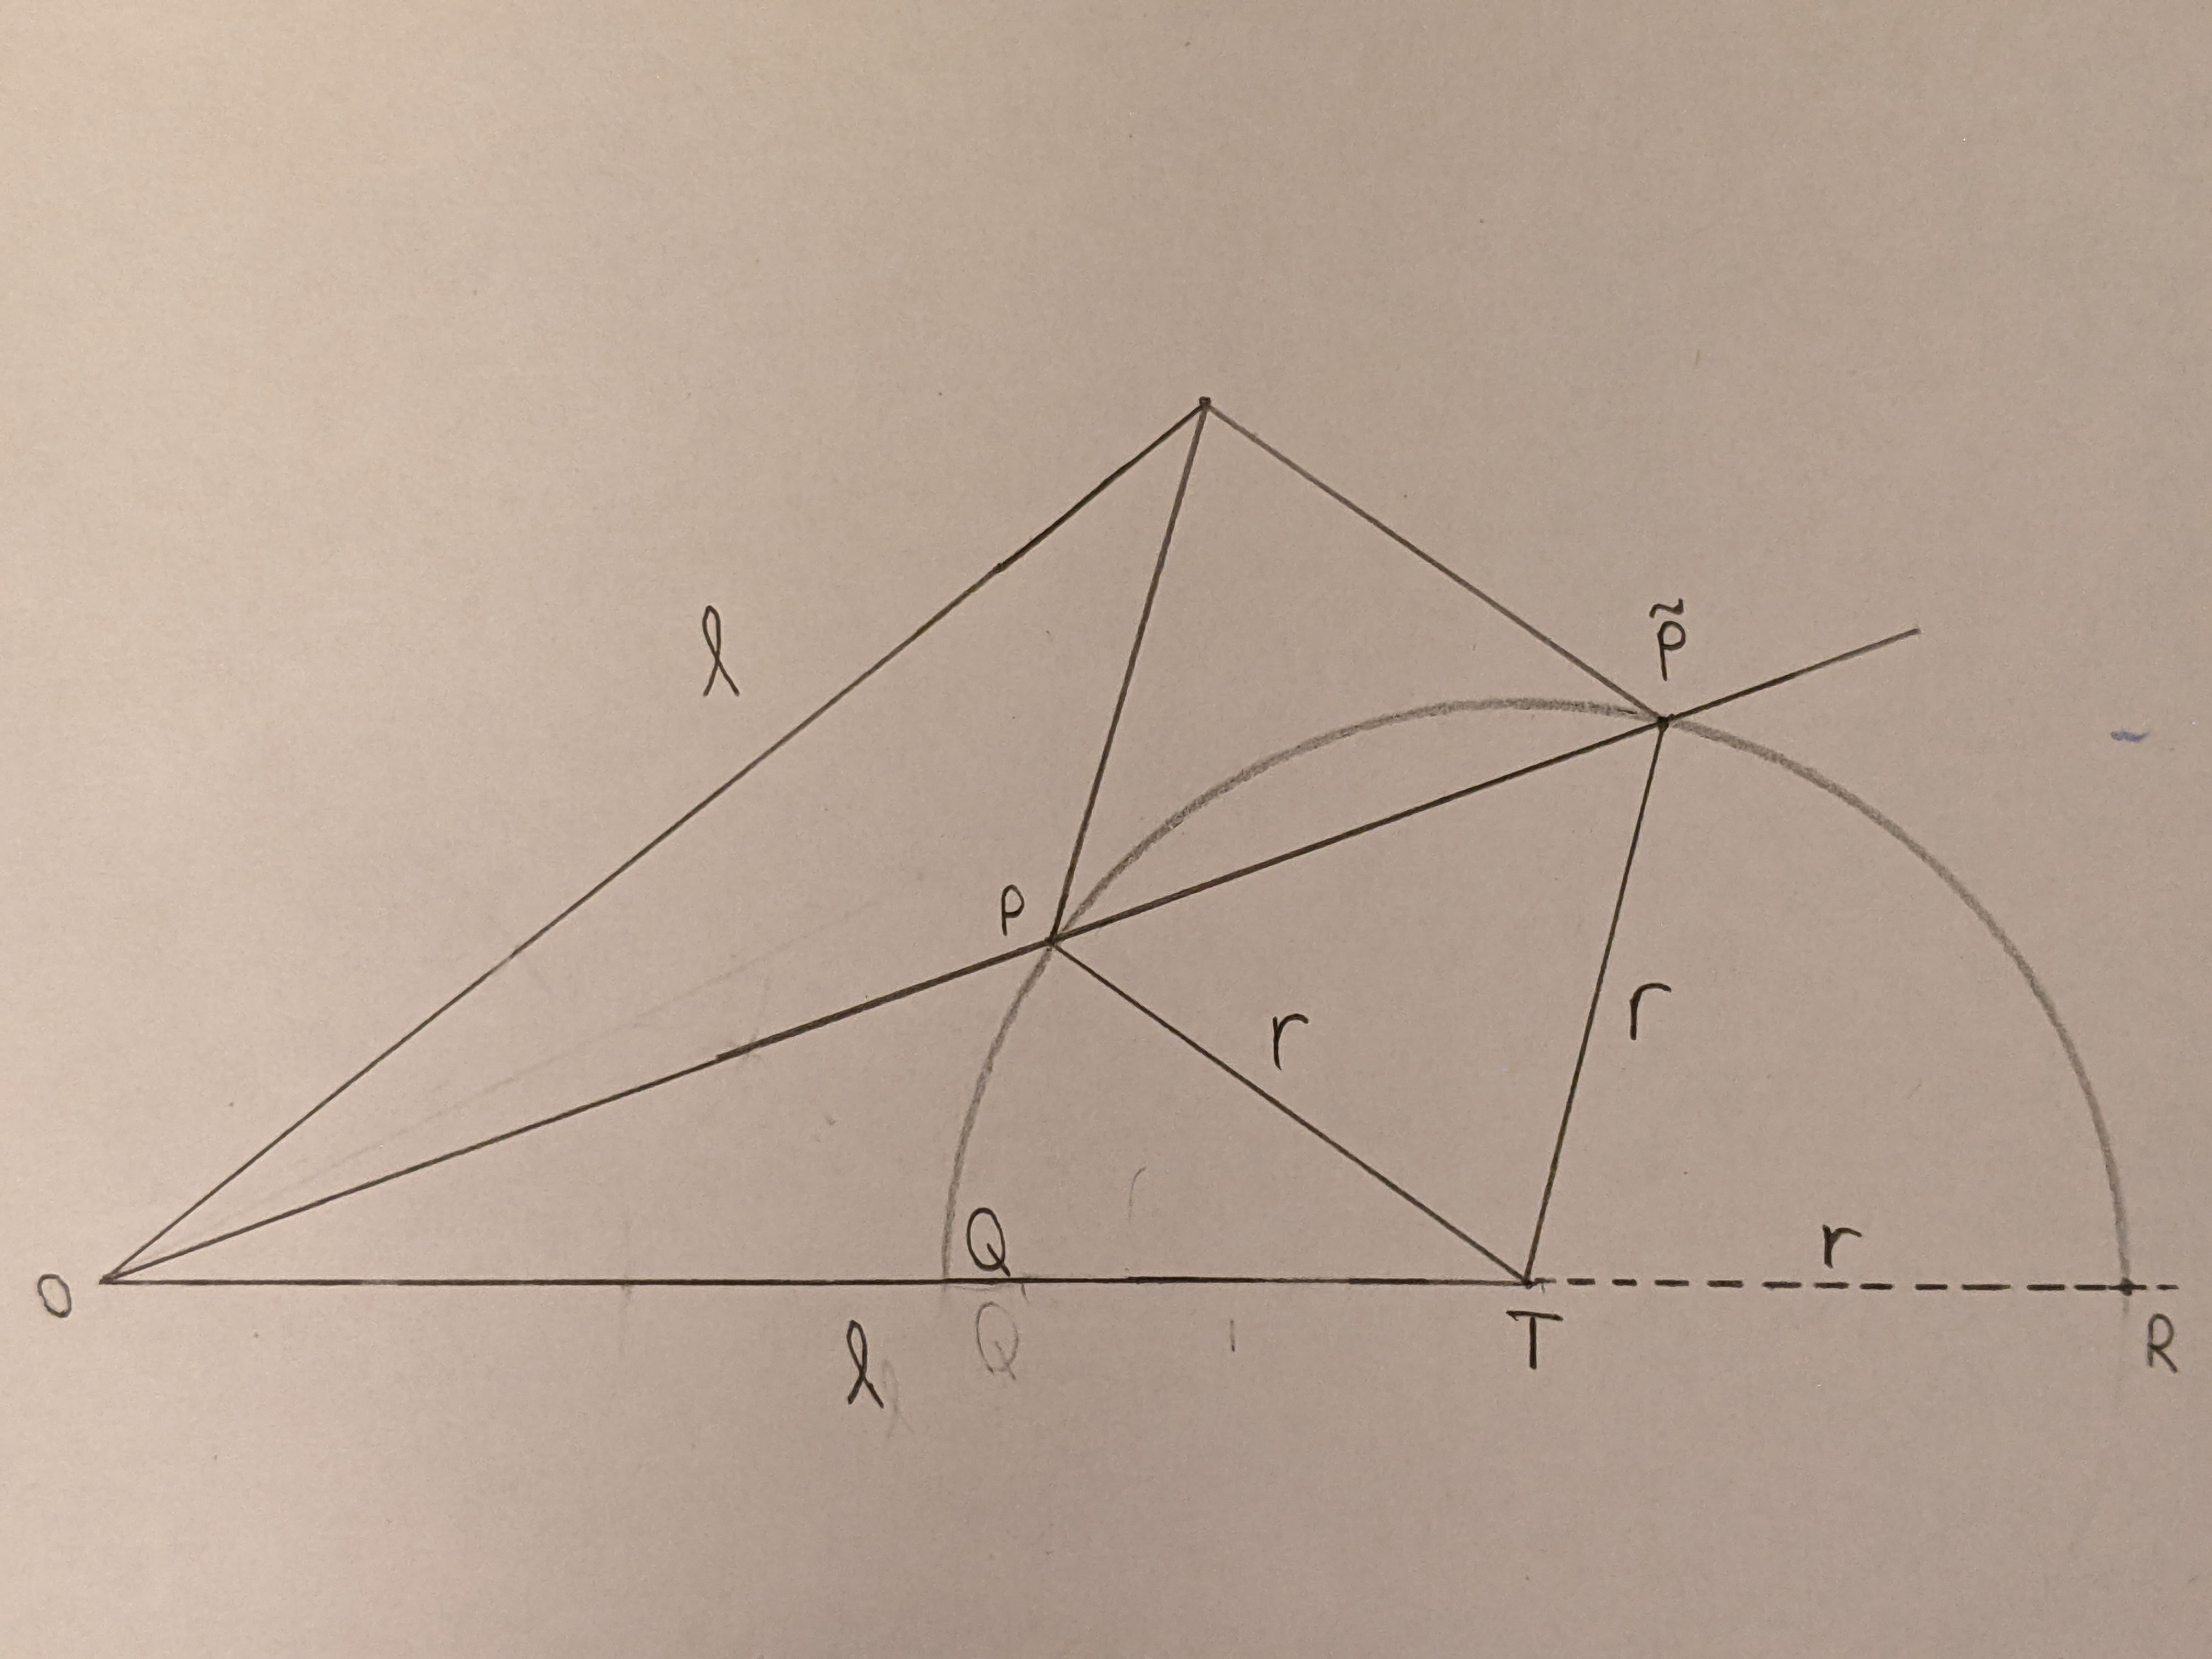
\includegraphics[width=\textwidth]{Problem2Image1}
\end{figure} 
\newpage
\section*{Chapter 3 Problem 5}
Let us consider the below image. We are examining a vertical slice of the Riemann sphere $\Sigma$ that contains the point $\alpha$, which is on the complex plane. The point $\beta$ is the image of $\alpha$ under the stereographic projection from the complex plane $\mathbb{C}$ to the Riemann sphere $\Sigma$. Then, $\gamma$ is the image of $\beta$ under stereographic projection from the south pole $S$ of the Riemann sphere $\Sigma$ to the complex plane $\mathbb{C}$. First, we will try to prove that $\angle \alpha \beta \gamma$ is a right angle. We know that $N = (0,1)$. Let $\alpha = (a,0)$. Then, the slope of the line connecting $\alpha$ to $N$ is 
\[
\frac{1-0}{0-a} = - \frac{1}{a}
\] Thus, the equation of the line connecting $\alpha$ and $N$ is
\[
y = -\frac{1}{a}x + 1
\] Let us substitute this value for $y$ into the equation $x^2+y^2 = 1$ to find the coordinates of the point $\beta$. We find that
\[
x^2 + \bigg(-\frac{1}{a}x + 1\bigg)^2 = 1
\] which is equivalent to
\[
x^2 + \frac{1}{a^2}x^2 - \frac{2}{a}x + 1 = 1
\] Simplifying, we obtain
\[
x(x(1+ 1/a^2)-2/a) = 0
\] One solution is when $x=0$, but this corresponds to the north pole $N$, so we may disregard it. Thus, we are left solving
\[
x(1+ 1/a^2)-2/a = 0
\] so that
\[
x = \frac{2/a}{1+1/a^2} = \frac{2/a}{1+1/a^2} \cdot \frac{a^2}{a^2} = \frac{2a}{a^2+1}
\] and 
\[
y = -\frac{1}{a}x + 1 = -\frac{1}{a} \cdot \frac{2a}{a^2+1} + 1 = -\frac{2}{a^2+1} + \frac{a^2+1}{a^2+1} = \frac{a^2-1}{a^2+1}
\] Thus, we know that
\[
\beta = \bigg(\frac{2a}{a^2+1}, \frac{a^2 - 1}{a^2 + 1}\bigg)
\] Next, we may compute the slope of the line connecting the south pole $S = (0,-1)$ and $\beta$ as follows:
\[
\frac{-1 - \frac{a^2 - 1}{a^2 + 1}}{0-\frac{2a}{a^2+1}} = \frac{\frac{-a^2 - 1 - (a^2 - 1)}{a^2+1}}{-\frac{2a}{a^2+1}} = \frac{\frac{-2a^2}{a^2+1}}{-\frac{2a}{a^2+1}} = \frac{-2a^2}{-2a} = a
\] Notice that 
\[
-\frac{1}{a} \cdot a = -1
\] so that the lines $\ell_1$ and $\ell_2$ are perpendicular; that is, $\angle \alpha \beta \gamma$ is a right angle. Since $\angle NO\alpha$ is also a right angle, we obtain $\angle \alpha \beta \gamma \cong \angle NO \alpha$. Furthermore, it is evident that $\angle \beta \alpha \gamma \cong \angle N \alpha O$. By angle-angle similarity, we may deduce that $\triangle NO \alpha \sim \triangle \gamma \beta \alpha$. This informs us that $\angle \alpha \gamma \beta \cong \angle ON\alpha$. Furthermore, we know that $\angle \alpha \gamma \beta \cong \angle S \gamma O$, so we may deduce that $\angle ON\alpha \cong \angle S \gamma O$. It is also evident that $\angle NO\alpha \cong \angle SO\gamma$. By angle-angle similarity, we may deduce that $\triangle S\gamma O \sim \triangle \alpha N O$. By triangle similarity, we know that 
\[
\frac{\vert OS \vert}{\vert O\gamma \vert} = \frac{\vert O\alpha \vert}{\vert ON \vert}
\] so that $\vert O \gamma \vert \vert O \alpha \vert  = \vert OS \vert \vert ON \vert = 1$ since $\vert ON \vert = \vert OS \vert = 1$. In particular, we find that $\vert \alpha \vert \vert \gamma \vert = 1$. Since $\gamma$ has the same argument as $\alpha$, we may deduce that $\gamma$ is the inverse of $\alpha$ over the unit circle. Thus, we may conclude that $f(z) = 1/\overline{z}$.
\begin{figure}[H]
\centering
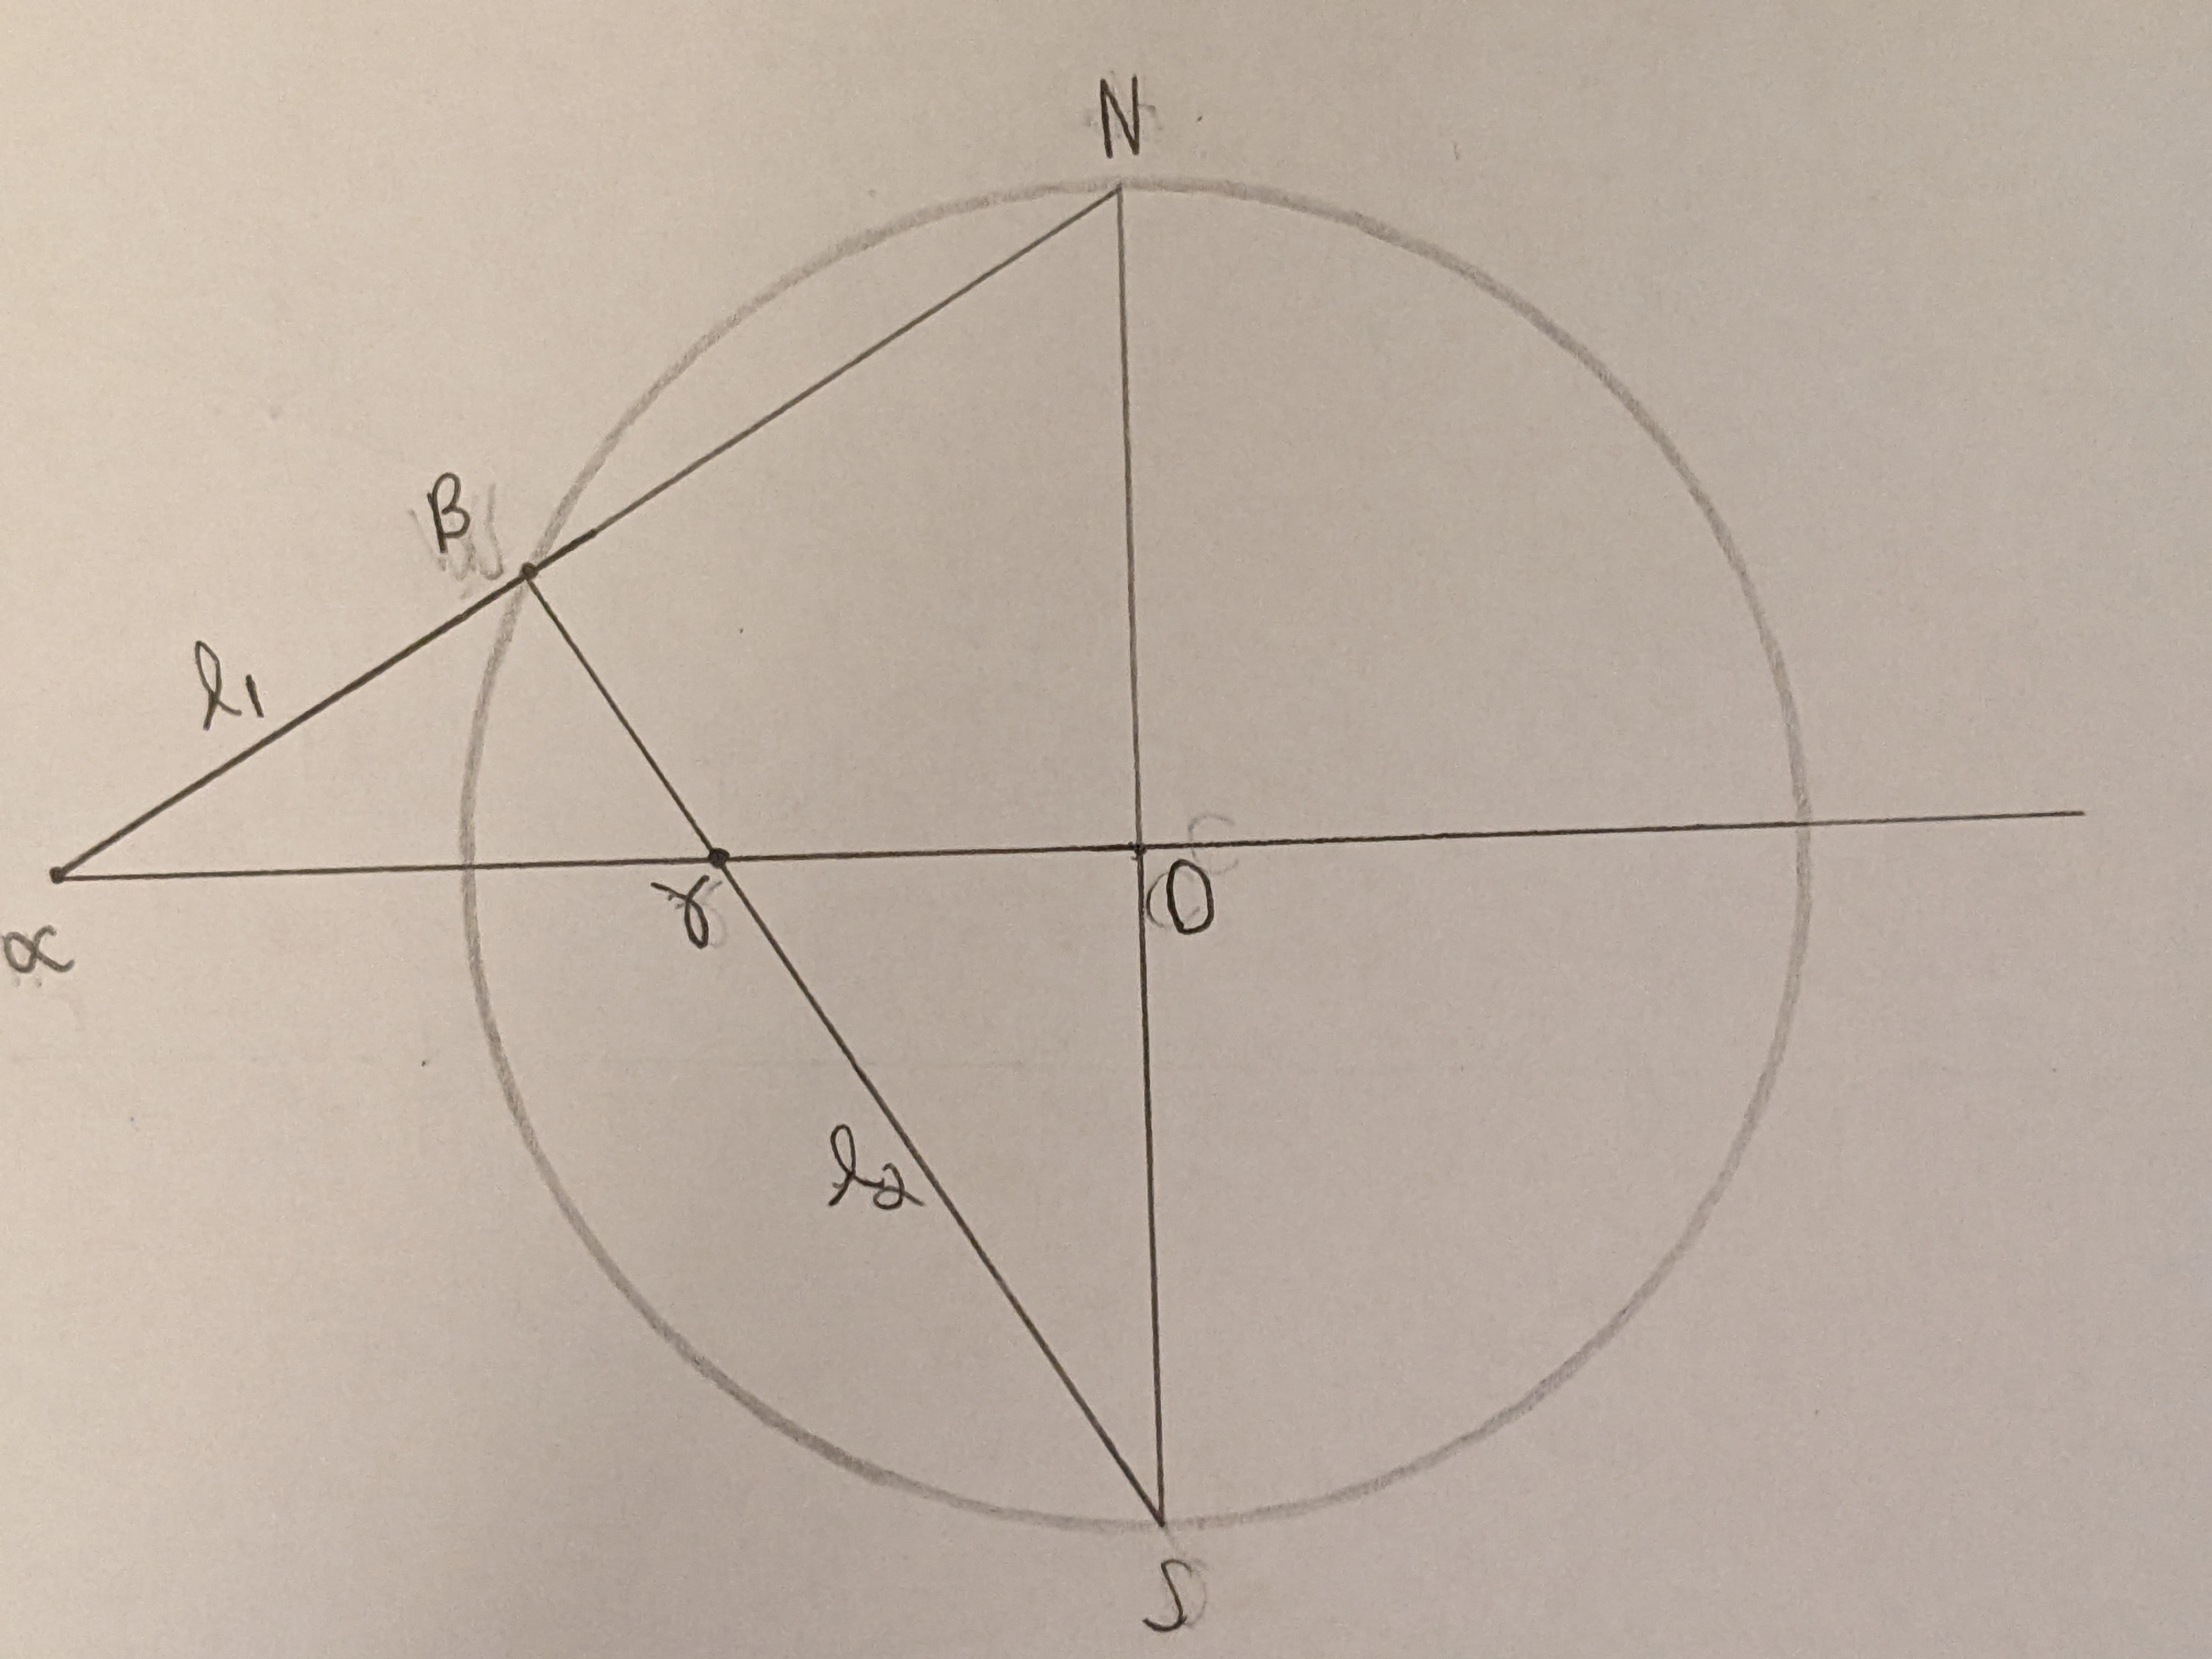
\includegraphics[width=\textwidth]{Problem5Image1}
\end{figure} 
\newpage
\section*{Chapter 2 Problem 16}
Notice that $(1-z)^{-m}$ is equal to
\[
1 + (-m)(-z) + \frac{-m(-m-1)}{2}(-z)^2 + \frac{-m(-m-1)(-m-2)}{3!}(-z)^3 + \cdots 
\] which is equal to
\[
1 + mz + \frac{m(m+1)}{2}z^2 + \frac{m(m+1)(m+2)}{3!}z^3 +  \frac{m(m+1)(m+2)(m+3)}{3!}z^4  
\] Notice that
\[
\binom{m+r-1}{r} = \frac{(m+r-1)!}{r!(m+r-1-r)!} = \frac{(m+r-1)!}{r!(m-1)!} = \frac{(m-1)!m\cdots (m+r-1)}{r!(m-1)!} = \frac{m \cdots (m+r-1)}{r!}
\] This corresponds to the coefficients in the binomial expansion that we computed above, so we obtain
\[
(1-z)^{-m} = \sum_{r=0}^\infty c_r z^r = \sum_{r = 0}^\infty \binom{m+r-1}{r} z^r
\]
\subsection*{Part I}
The reason why $c_9$ is the number of distinguishable rearrangements of this sequence of $11$ symbols is because for each rearrangement, we obtain a copy of $z^9$ from the product $(1-z)^{-3}$ (and $c_9$ counts the number of copies of $z^9$ from this product). If the sequence is of the form $\bullet z \cdots$, then this copy of $z^9$ is obtained by multiplying $1$ from the first $(1-z)^{-1}$ term by one element each from the other two copies of $(1-z)^{-1}$. If the sequence is of the form $\cdots z \bullet$, then this copy of $z^9$ is obtained by multiplying $1$ from the last $(1-z)^{-1}$ term by one element each from the other two copies of $(1-z)^{-1}$. If the sequence is of the form $z\cdots \bullet \bullet \cdots z$, then this copy of $z^9$ is obtained by multiplying $1$ from the middle $(1-z)^{-1}$ term by one element each from the other two copies of $(1-z)^{-1}$.
\subsection*{Part II}
Recall that $c_9$ counts the number of ways of arranging $9$ $z$'s and $2$ $\bullet$'s. We are essentially choosing $9$ of the symbols in a string with $11$ characters to be $z$'s. Thus, we know that
\[
c_9 = \binom{11}{9}
\]
\subsection*{Part III}
Let $m$ and $r$ be fixed. To find $c_r$, we must count the number of ways of obtaining $z^r$ from the product $(1-z)^{-m}$. As above, this is counting the number of arrangements of $z$'s and $\bullet$'s. The number of $z$'s is $r$, and the number of $\bullet$'s is $m-1$. Thus, we must choose $r$ of the $m+r-1$ symbols to be $z$'s. Thus, we find that
\[
c_r = \binom{m+r-1}{r}
\] and the theorem is proved.
\newpage
\section*{Chapter 3 Problem 16}
\subsection*{Part I}
As stated in the textbook, $[z,q,r,s]$ represents the Mobius transformation that takes $q$ to $0$, $r$ to $1$, and $s$ to $\infty$. That is, it takes the first coordinate to $0$, the second coordinate to $1$, and the last coordinate to $\infty$. There are three options for the first coordinate, namely $q$, $r$, and $s$. Then, there are two options for the second coordinate and only one option for the last coordinate. These Mobius transformations are all different because there is only one Mobius transformation that takes any three points to $0$, $1$, and $\infty$.
\subsection*{Part II}
Let us first consider the following image:
\begin{figure}[H]
\centering
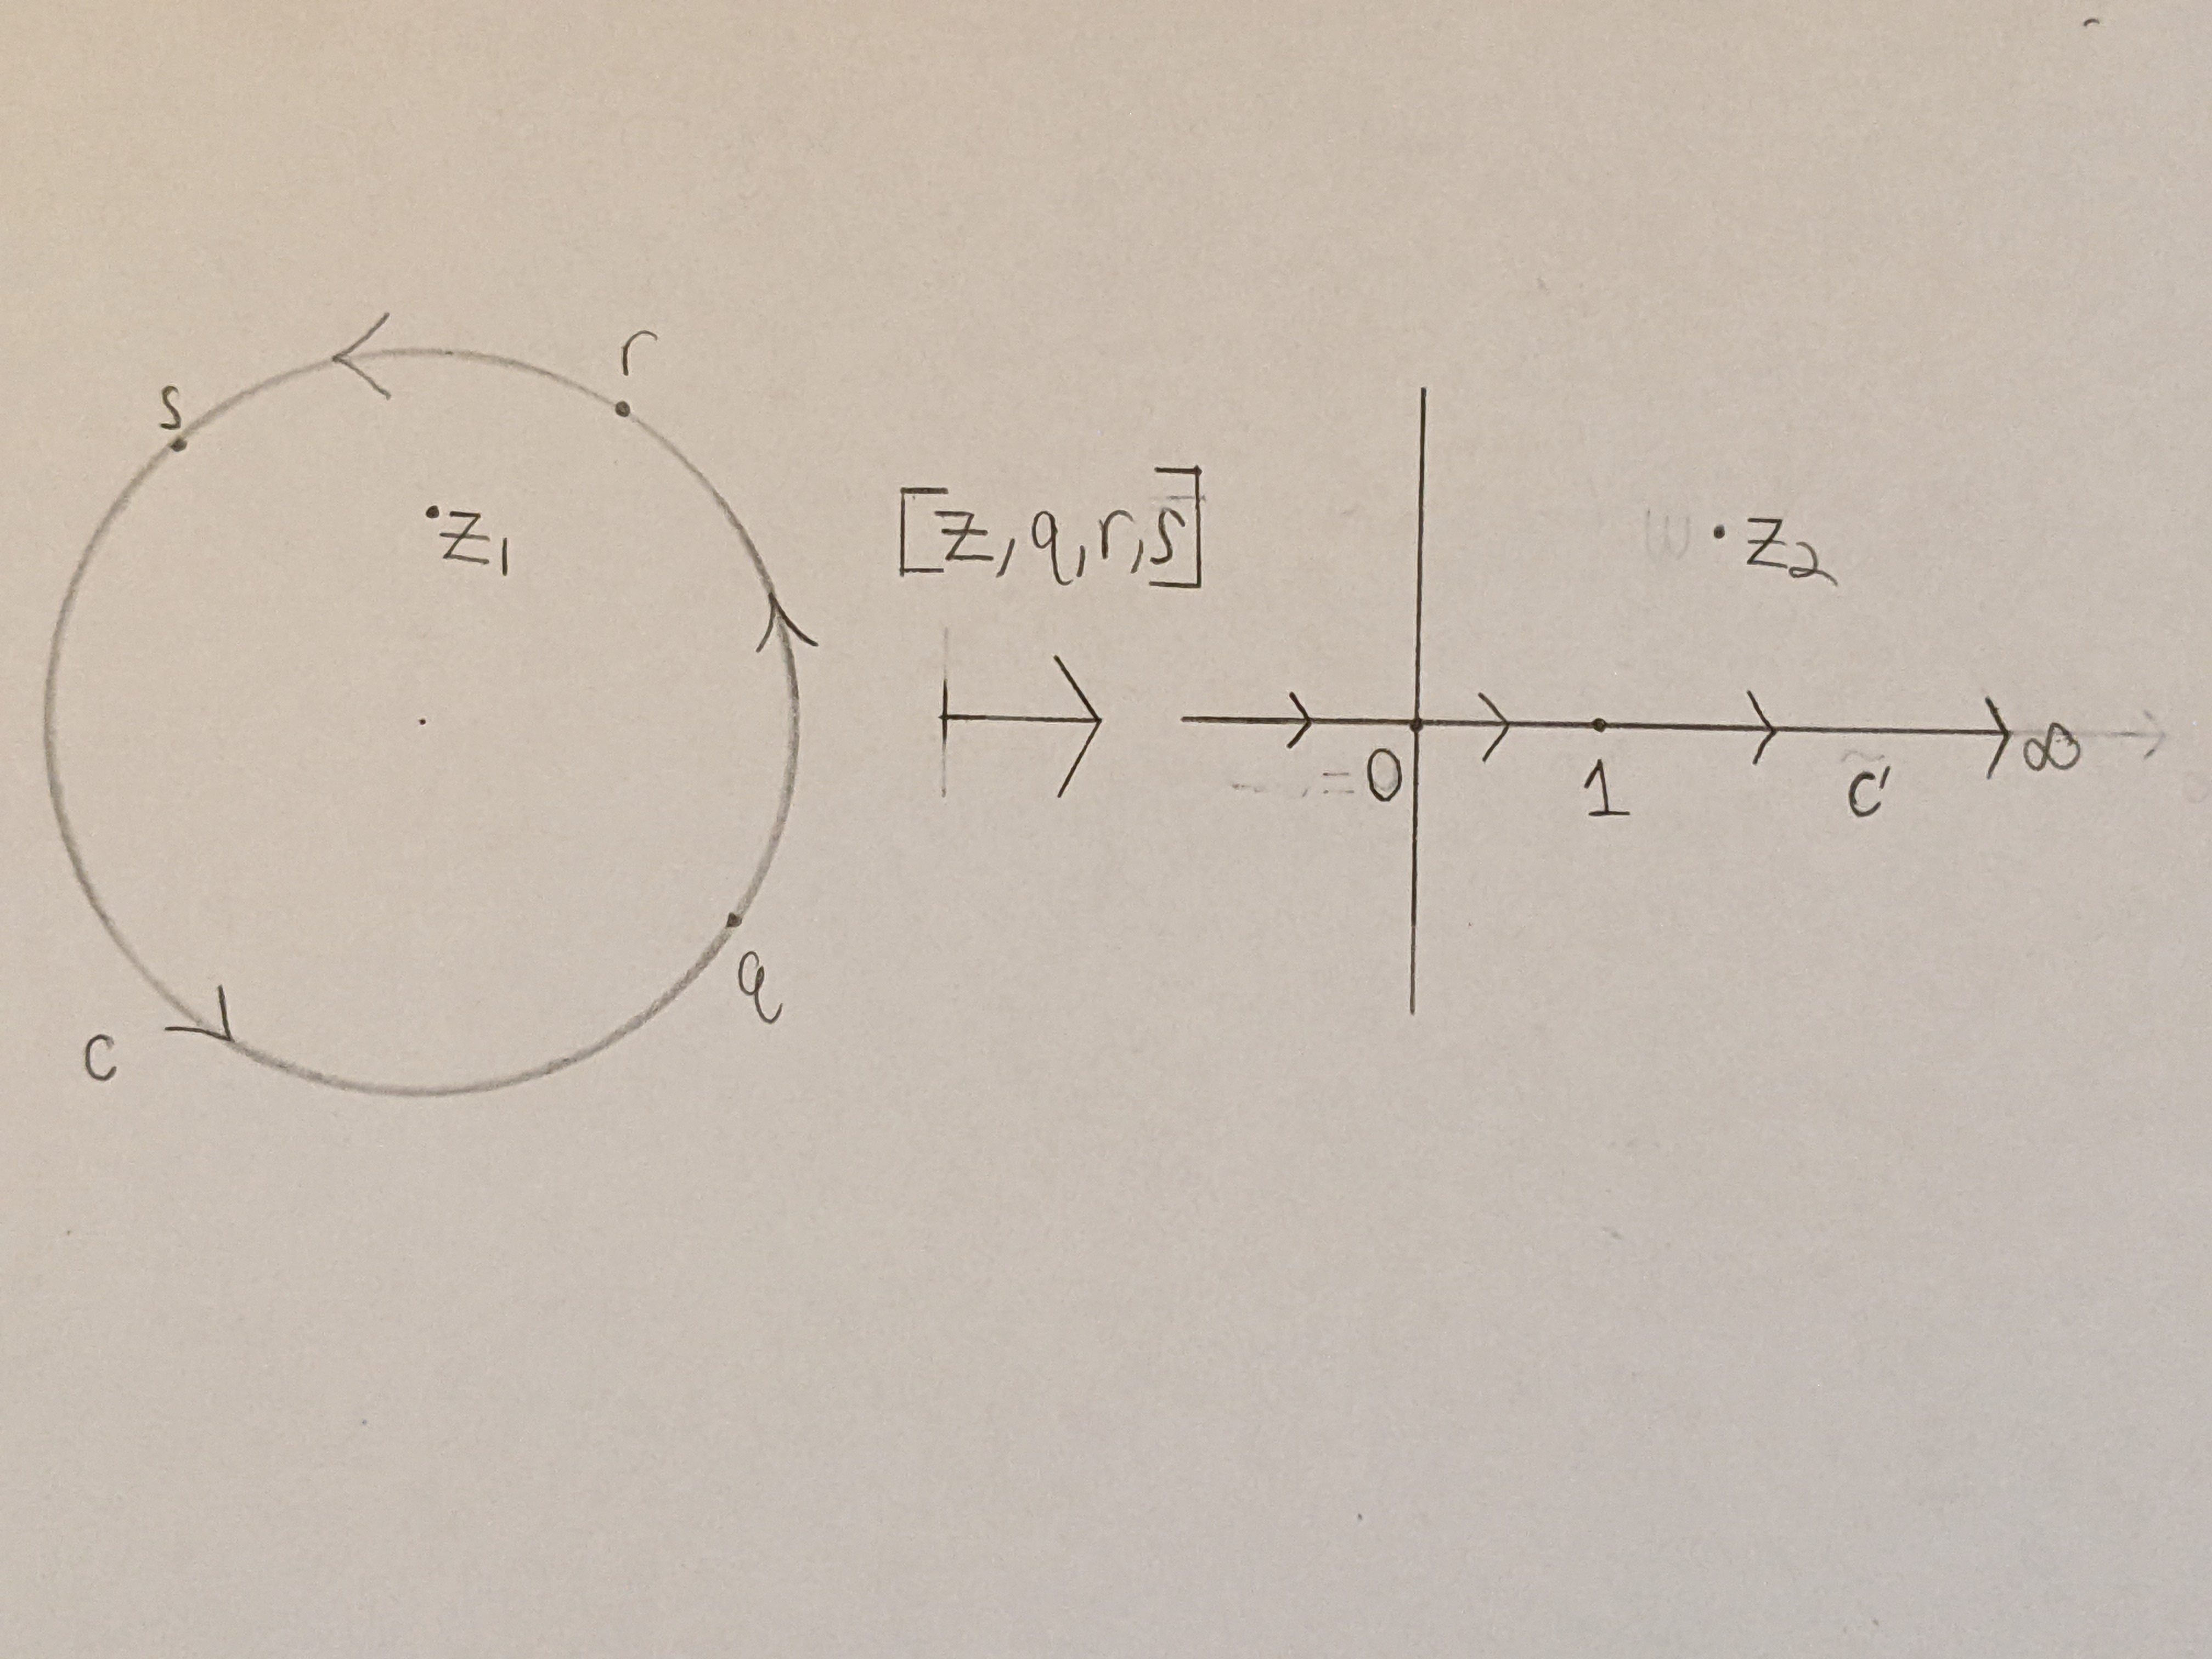
\includegraphics[width=\textwidth]{Problem16Image1}
\end{figure} 
\noindent In this image, $q$ is sent to $0$, $r$ is sent to $1$, and $s$ is sent to $\infty$. Furthermore, $z_1$ is sent to $z_2$, and $C$ is sent to $C^\prime$. Let us next consider the following image:
\begin{figure}[H]
\centering
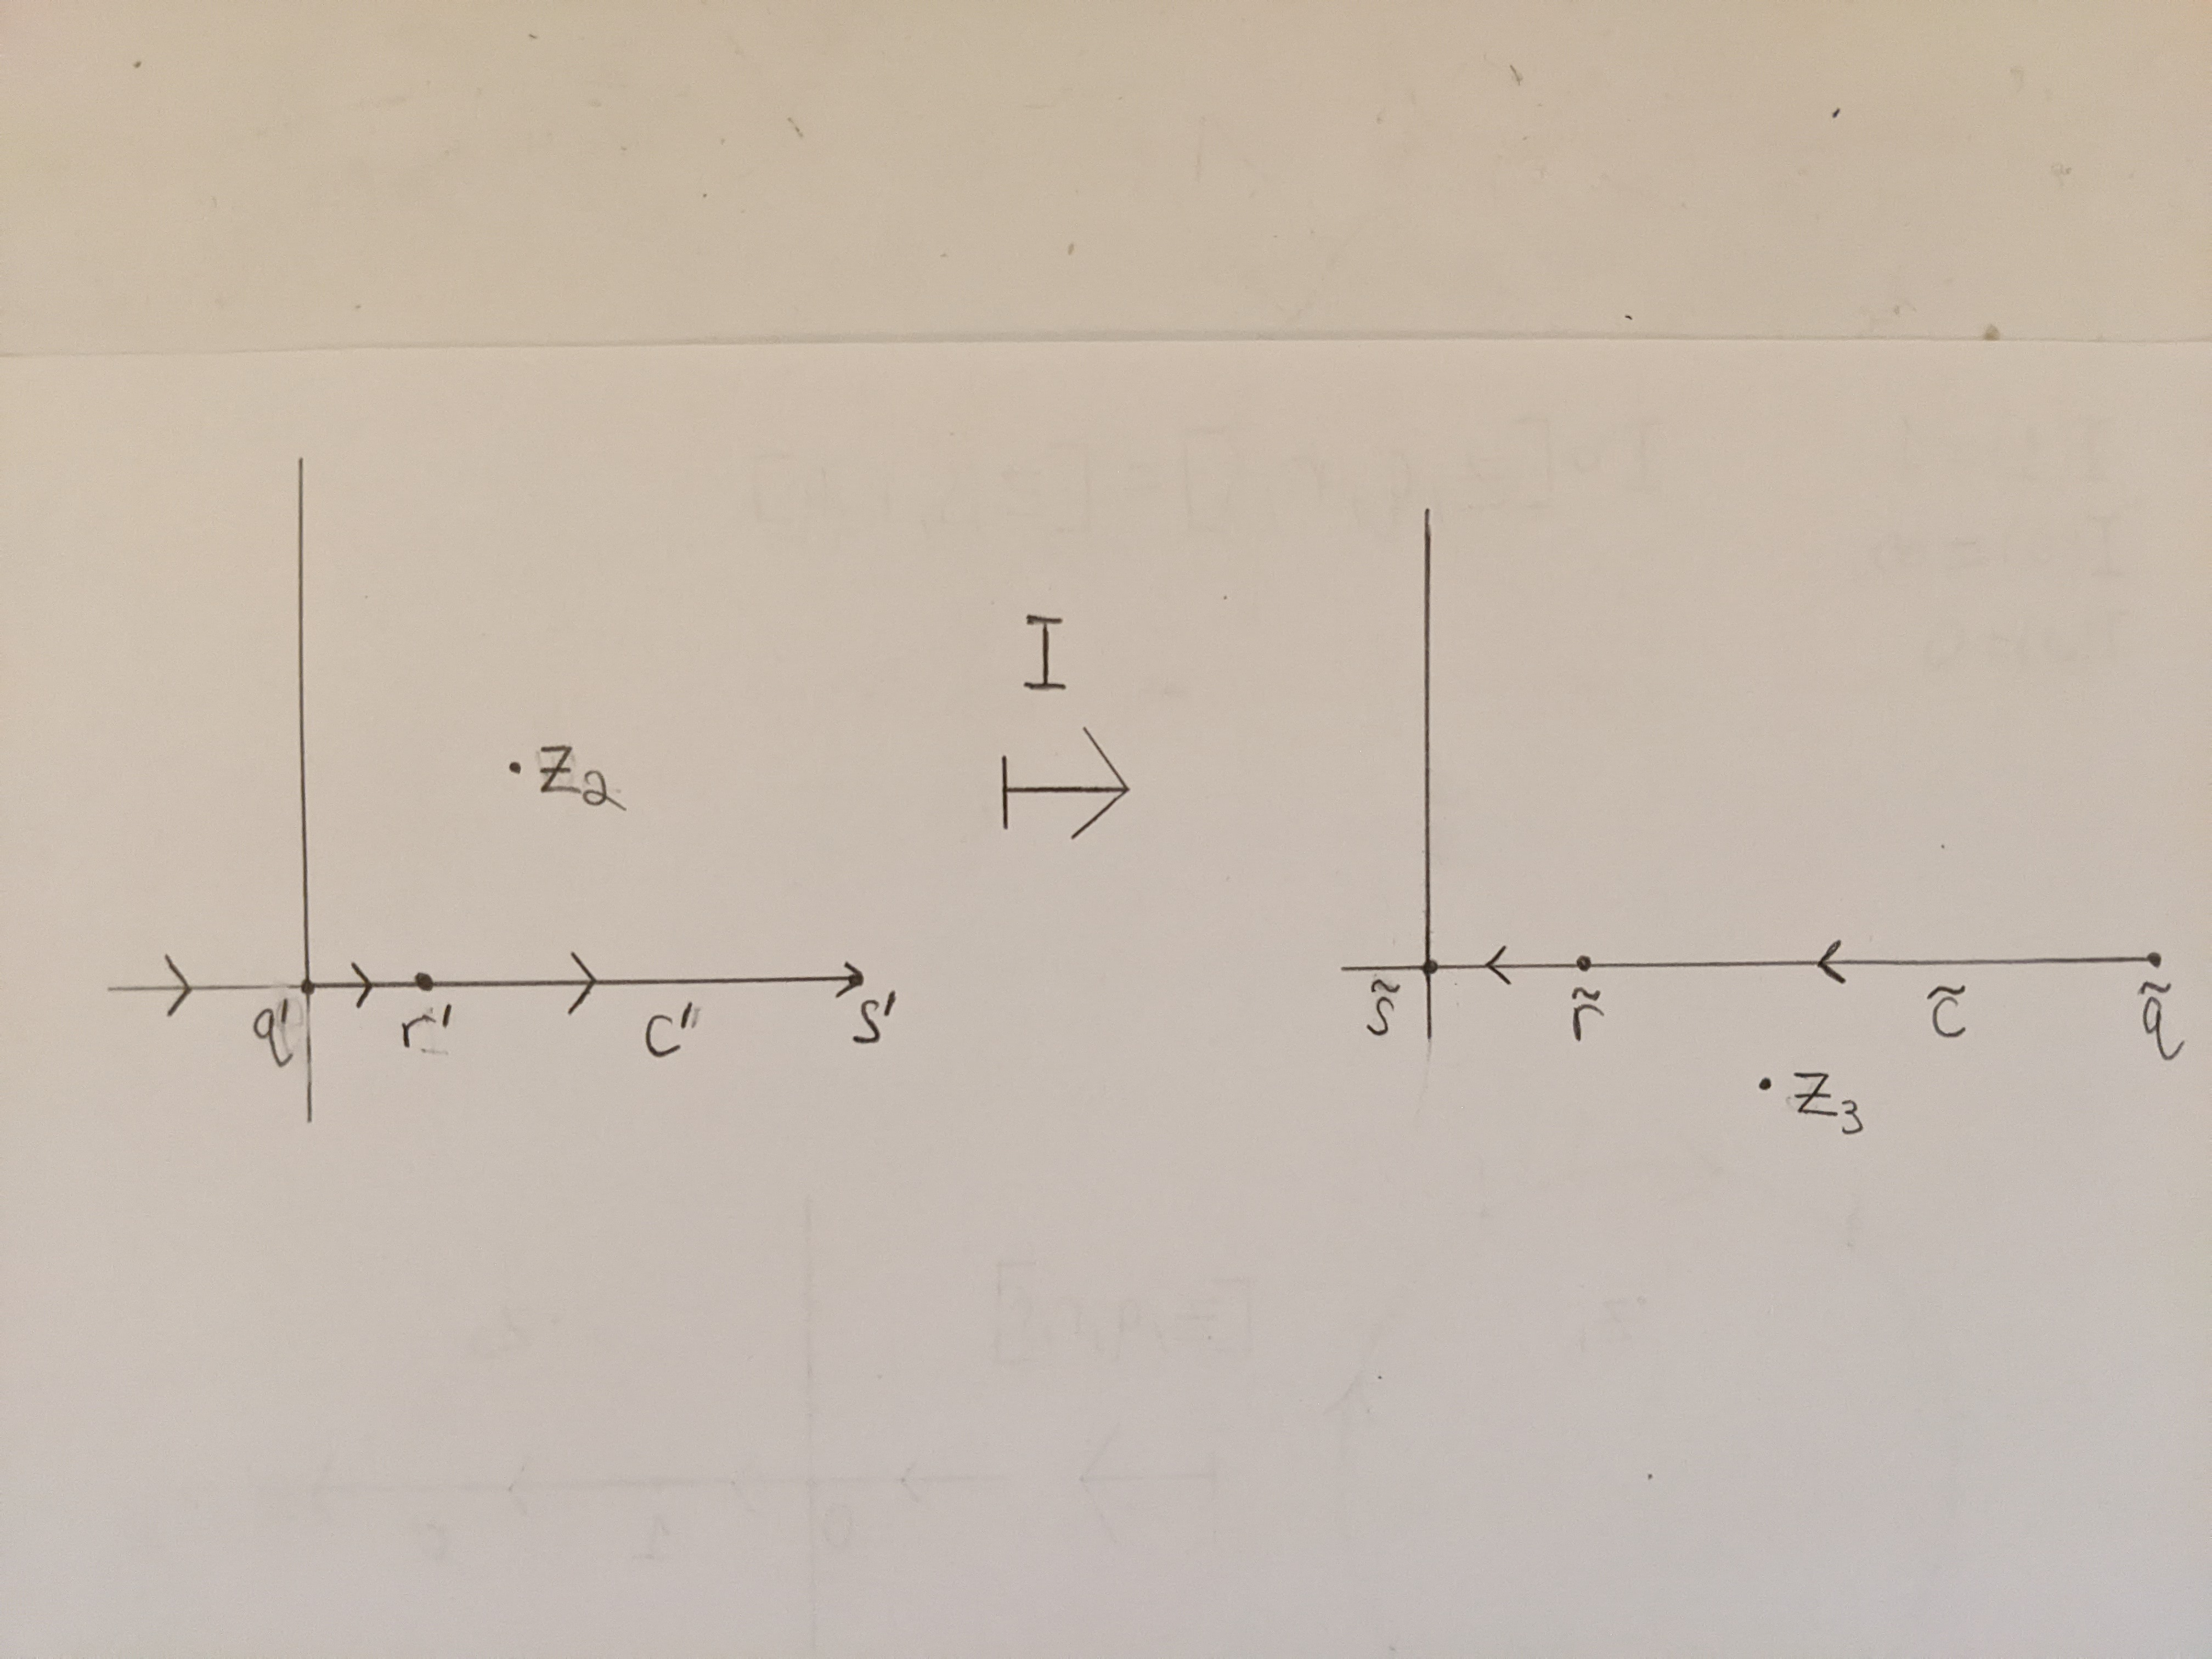
\includegraphics[width=\textwidth]{Problem16Image2}
\end{figure} 
\noindent Here, we have labeled $0$ as $q^\prime$, $1$ as $r^\prime$, and $\infty$ as $s^\prime$. The images of $q^\prime$, $r^\prime$, and $s^\prime$ under $I$ are $\tilde{q}$, $\tilde{r}$, and $\tilde{s}$. The image of $C^\prime$ is $\tilde{C}$, and the image of $z_2$ is $z_3$. Thus the composition $I\circ[z,q,r,s]$ takes $q$ to $\infty$, $r$ to $1$, and $s$ to $0$.
\begin{figure}[H]
\centering
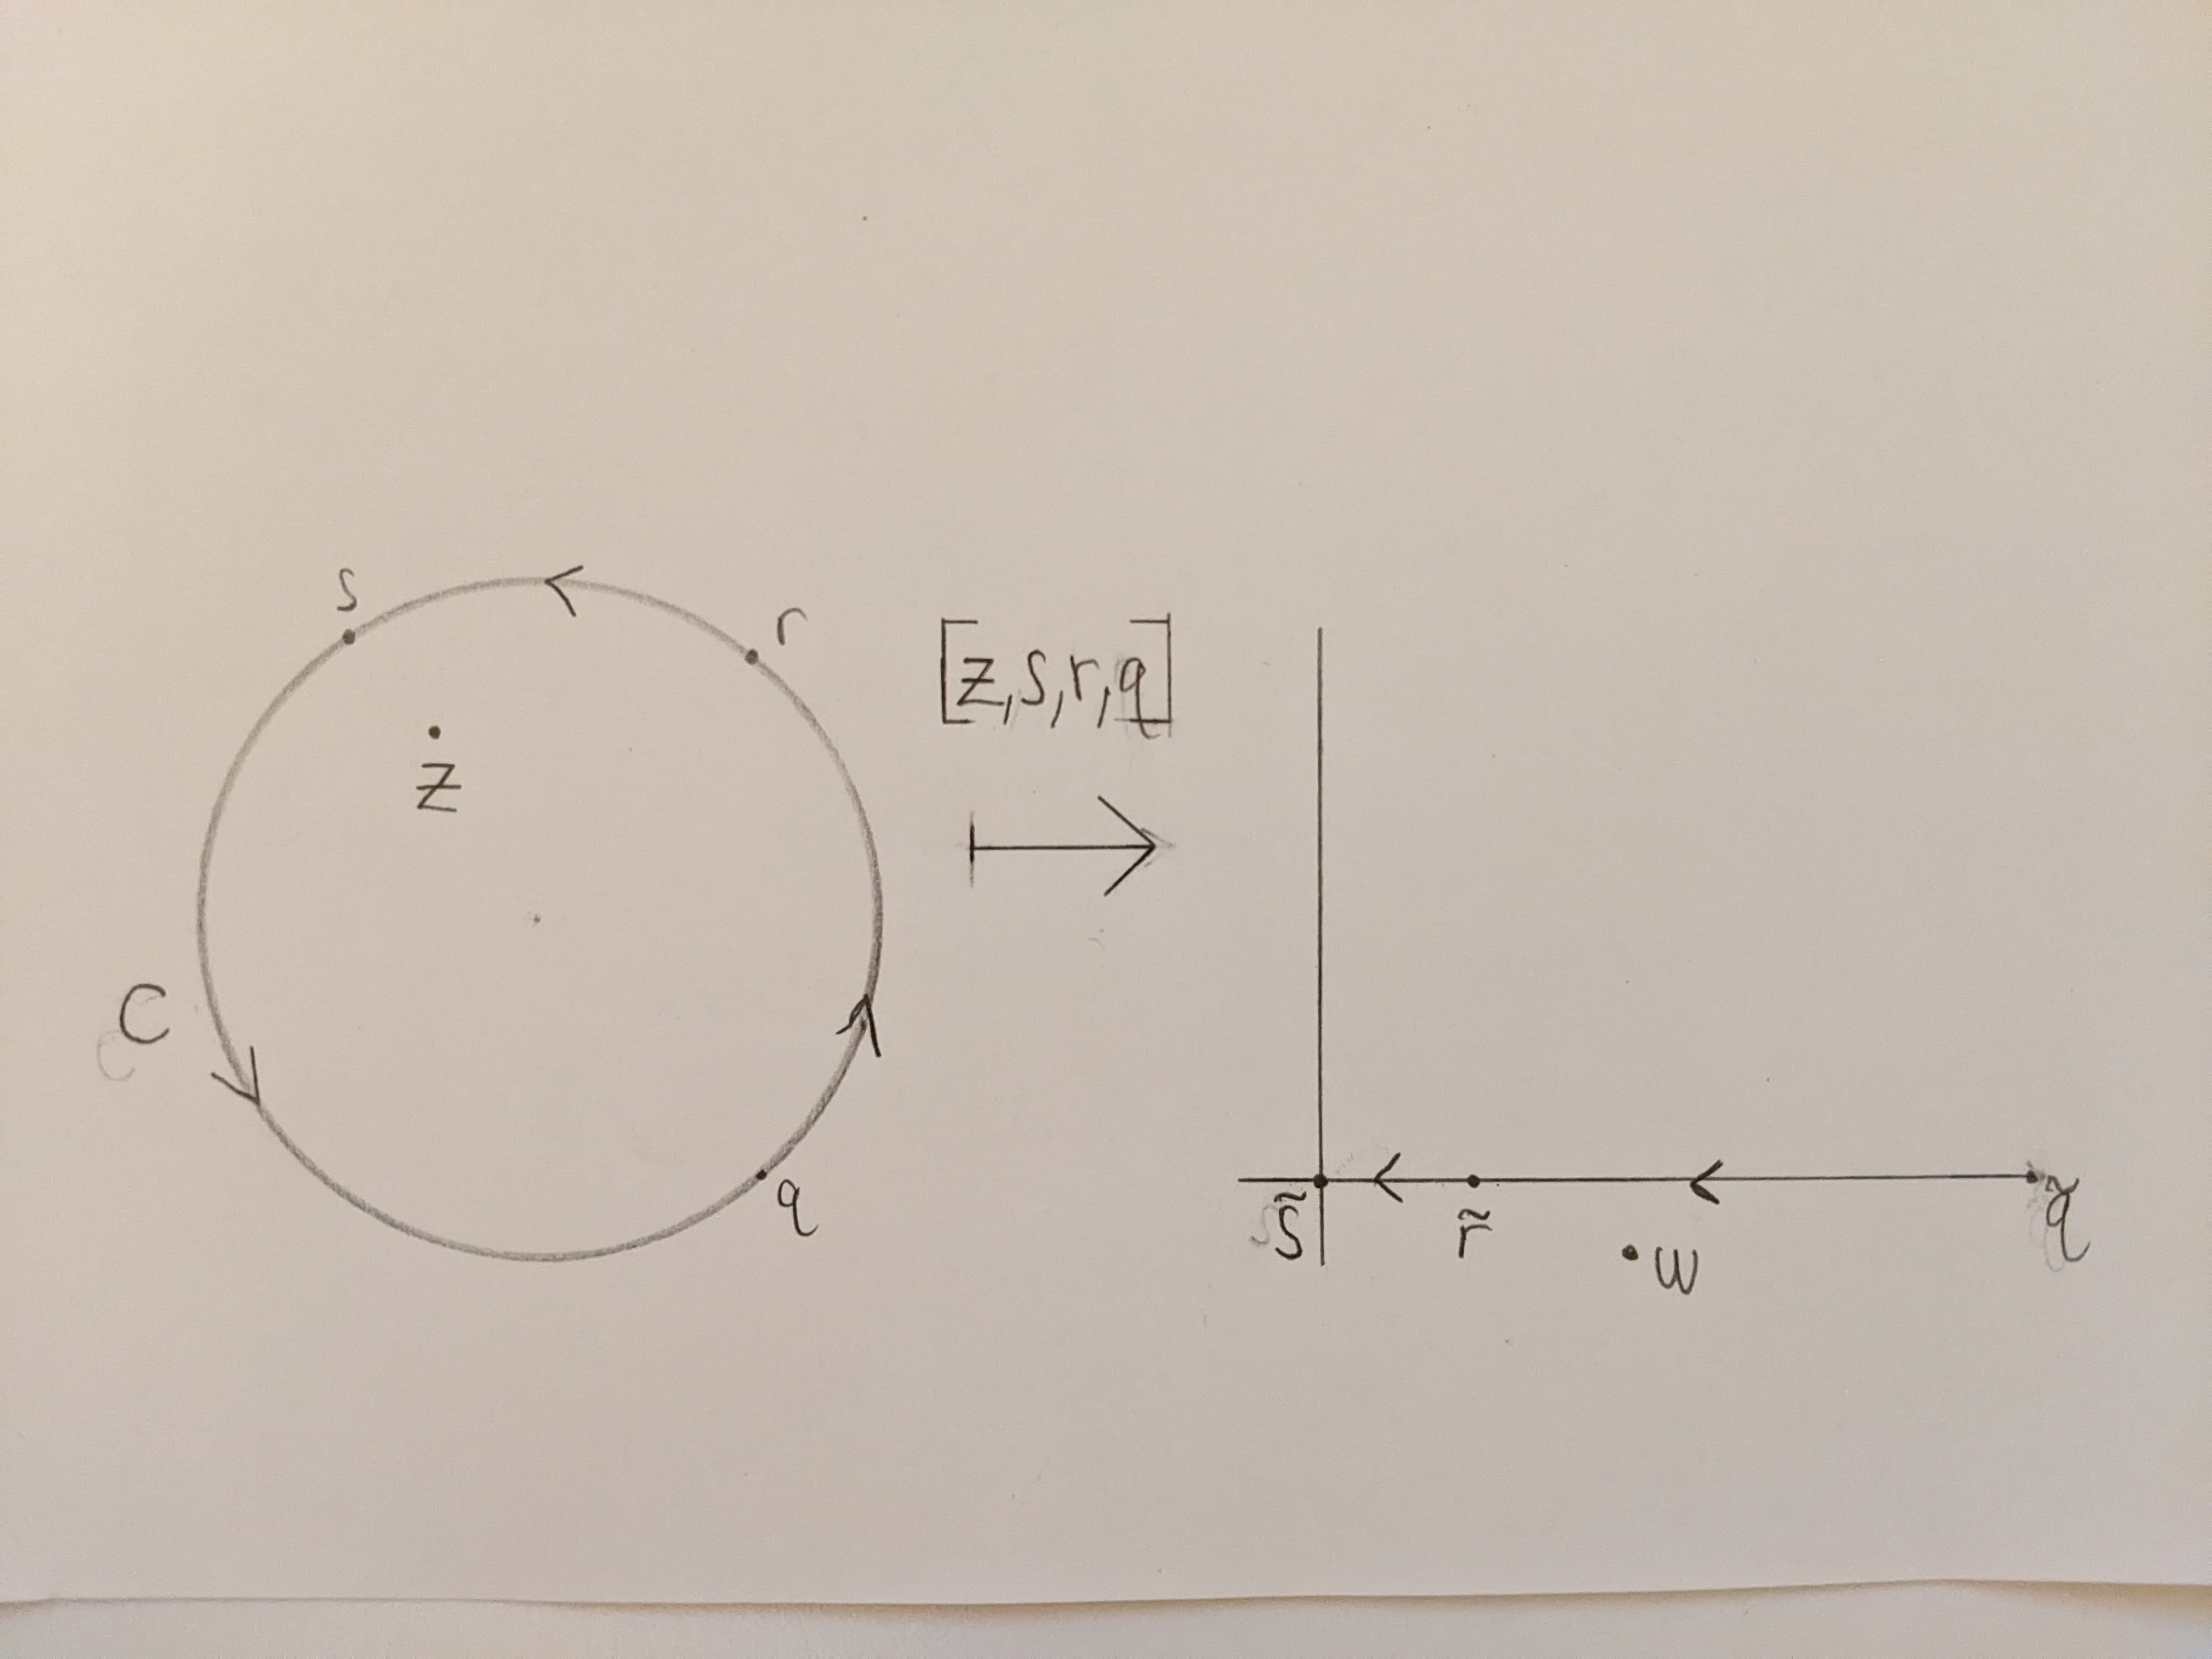
\includegraphics[width=\textwidth]{Problem16Image3}
\end{figure} 
\noindent Finally, we may consider the above image. In this image, $q$ is sent to $\infty$, $r$ is sent to $1$, and $s$ is sent to $0$. Since $I\circ[z,q,r,s]$ and $[z,s,r,q]$ agree on the three points $q$, $r$, and $s$, we may deduce that they are actually the same.
\subsection*{Part III}
Let us first consider the following image:
\begin{figure}[H]
\centering
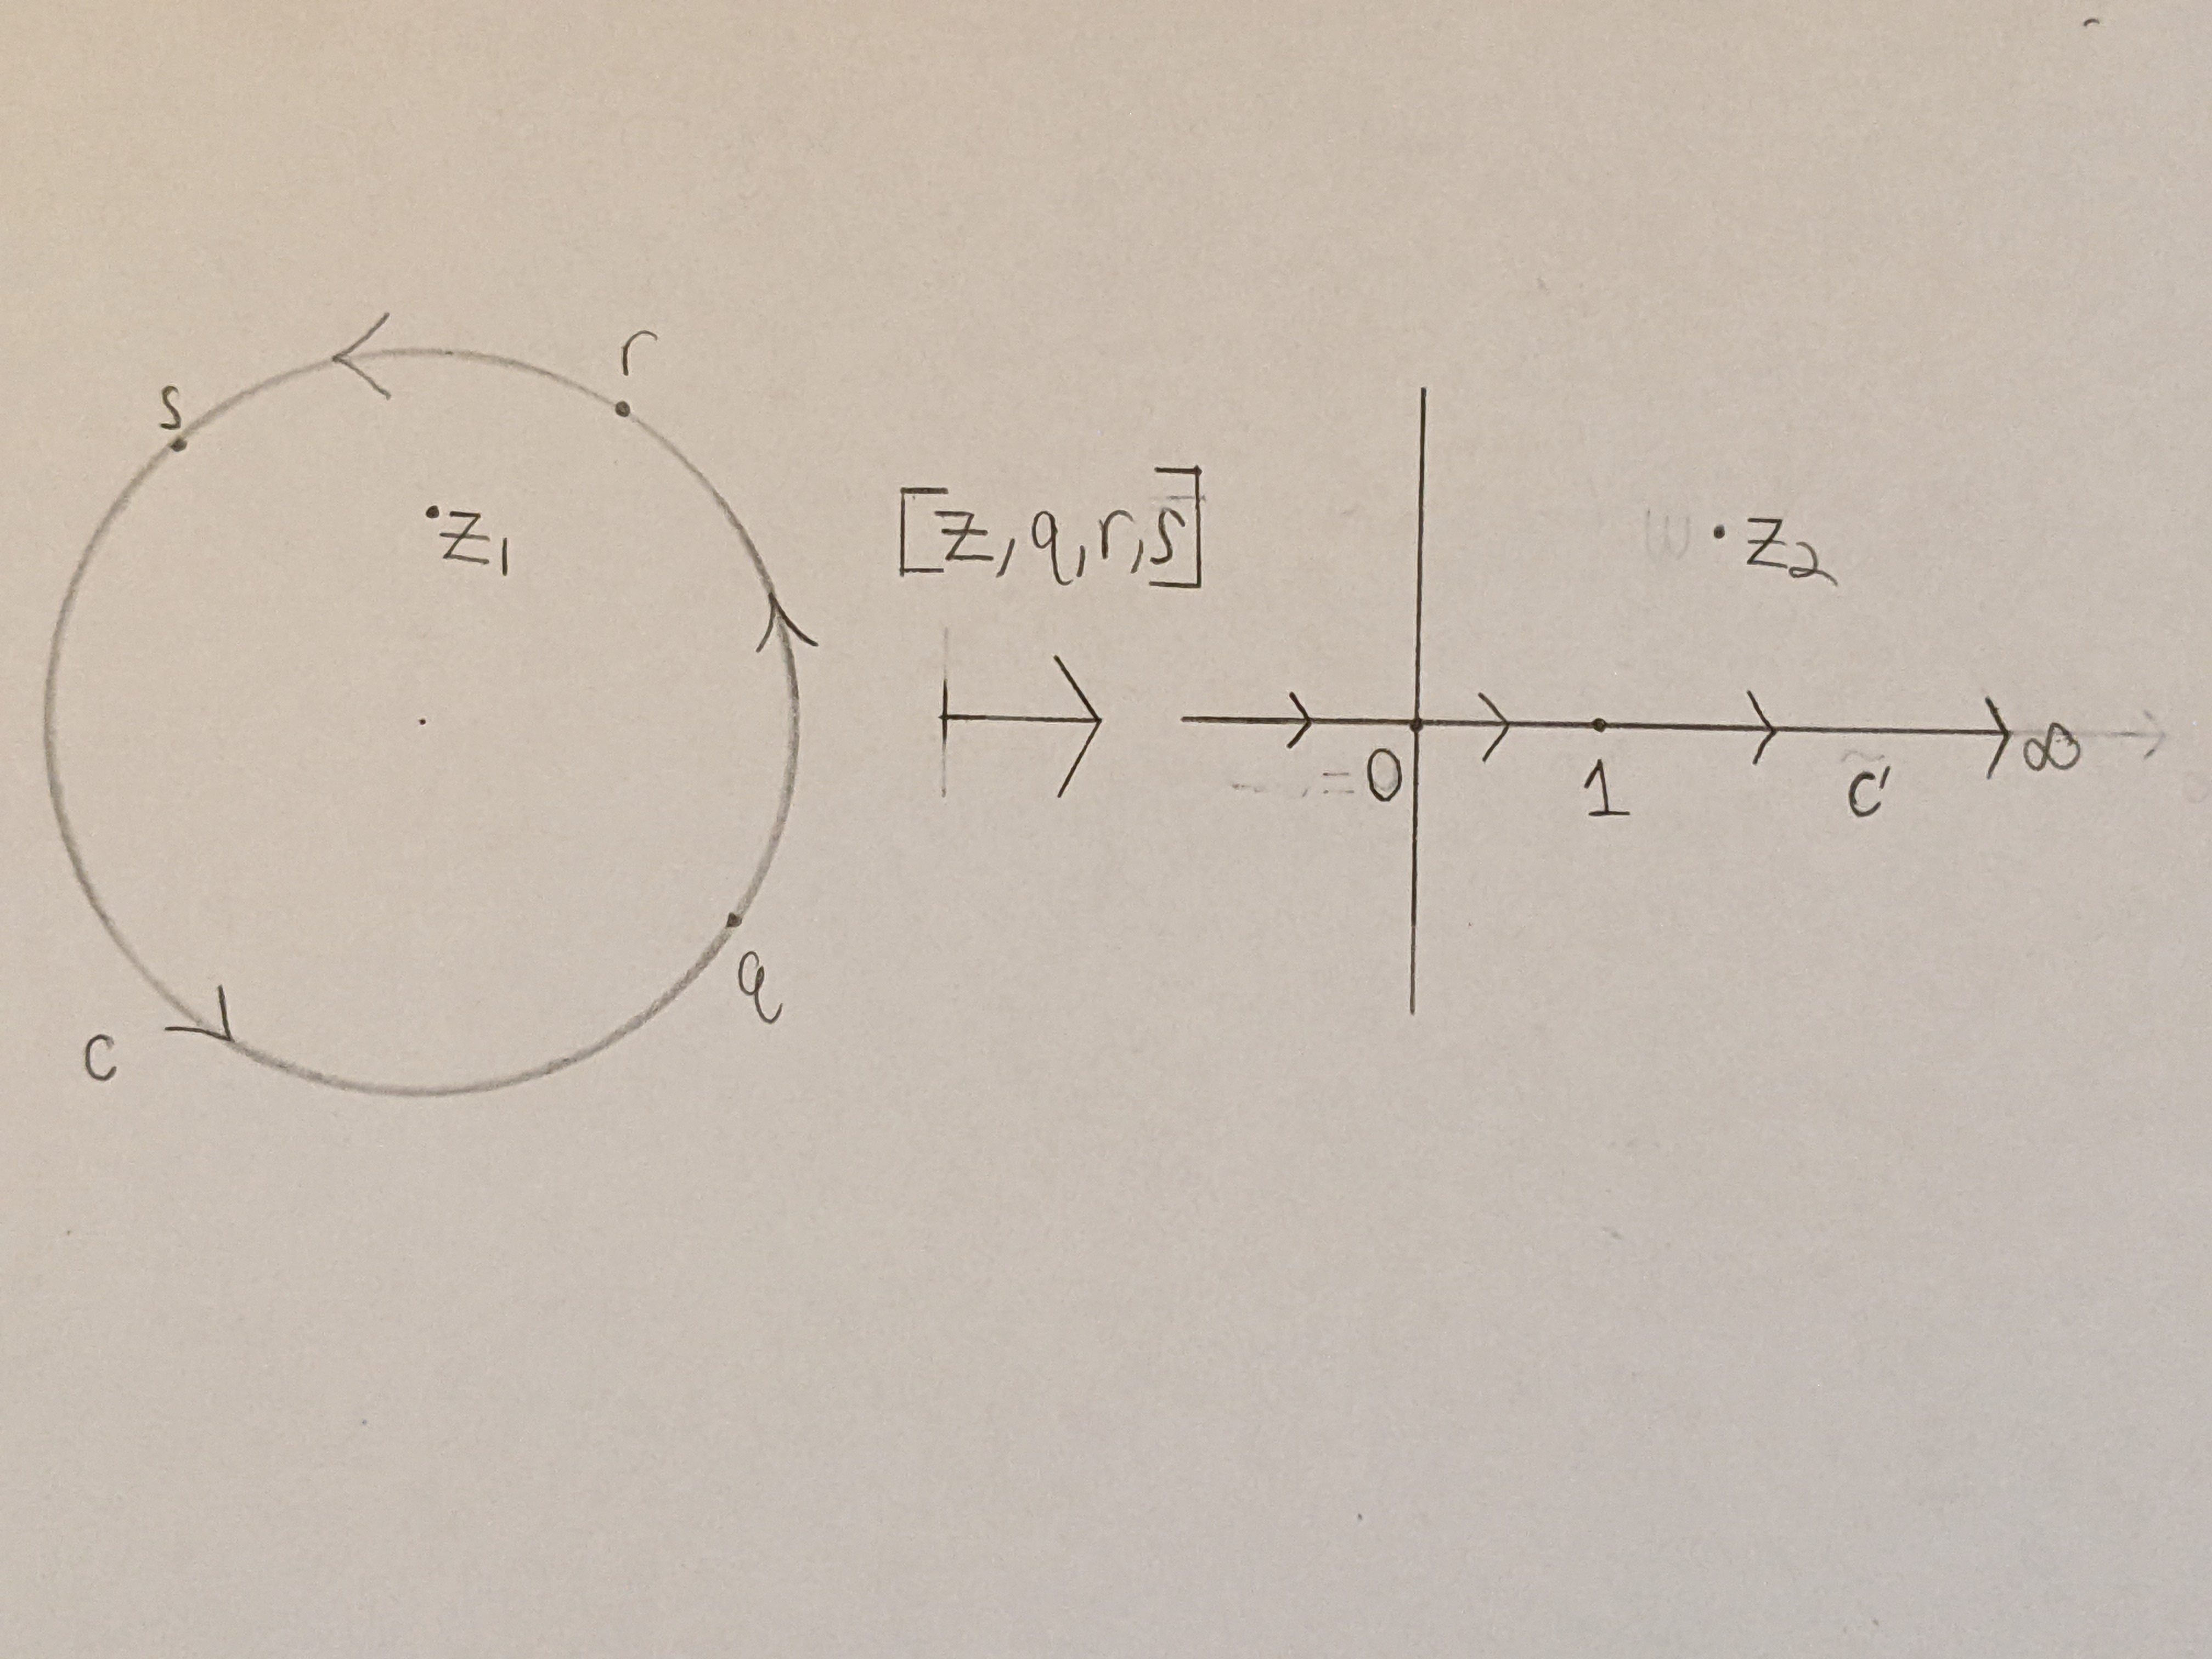
\includegraphics[width=\textwidth]{Problem16Image1}
\end{figure} 
\noindent Here $q$ is sent to $0$, $r$ is sent to $1$, and $s$ is sent to $\infty$. Next, we may consider the following image:
\begin{figure}[H]
\centering
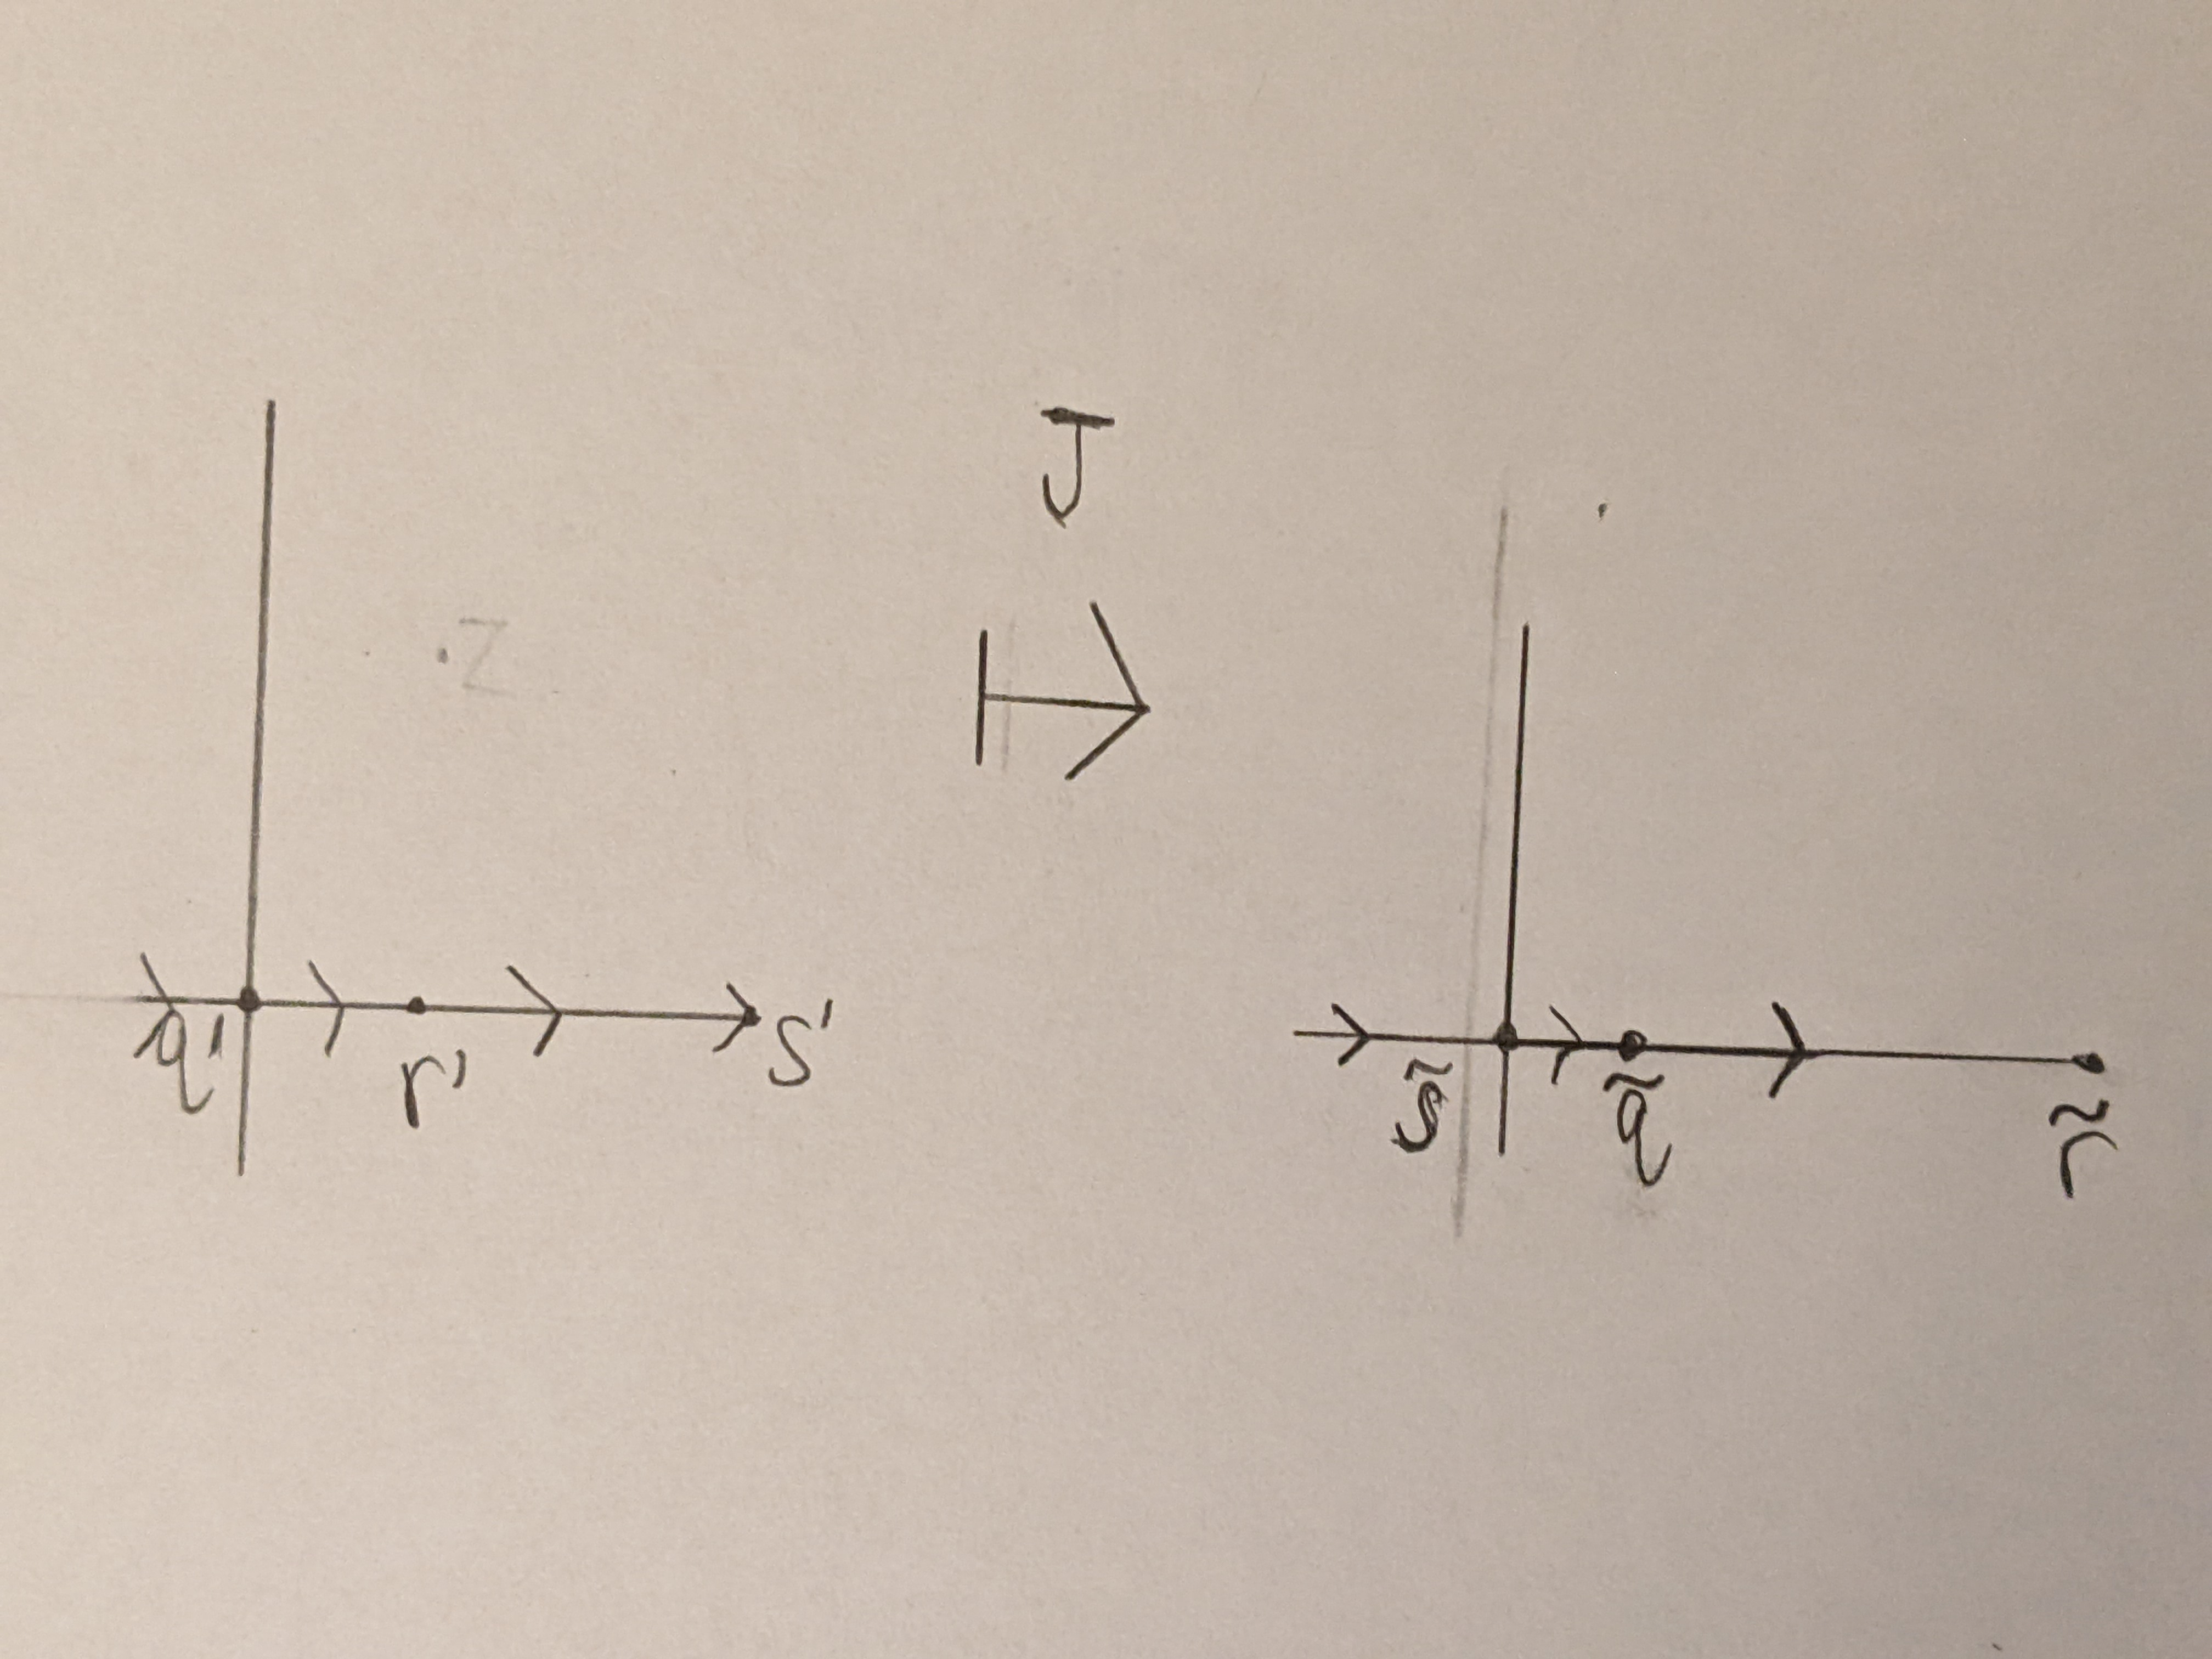
\includegraphics[width=\textwidth]{Problem16Image4}
\end{figure}
\noindent In this image, $q^\prime = 0$ is sent to $\tilde{q} = 1$, $r^\prime = 1$ is sent to $\tilde{r} = \infty$, and $s^\prime = \infty$ is sent to $\tilde{s} = 0$. Finally, let us consider the following image:
\begin{figure}[H]
\centering
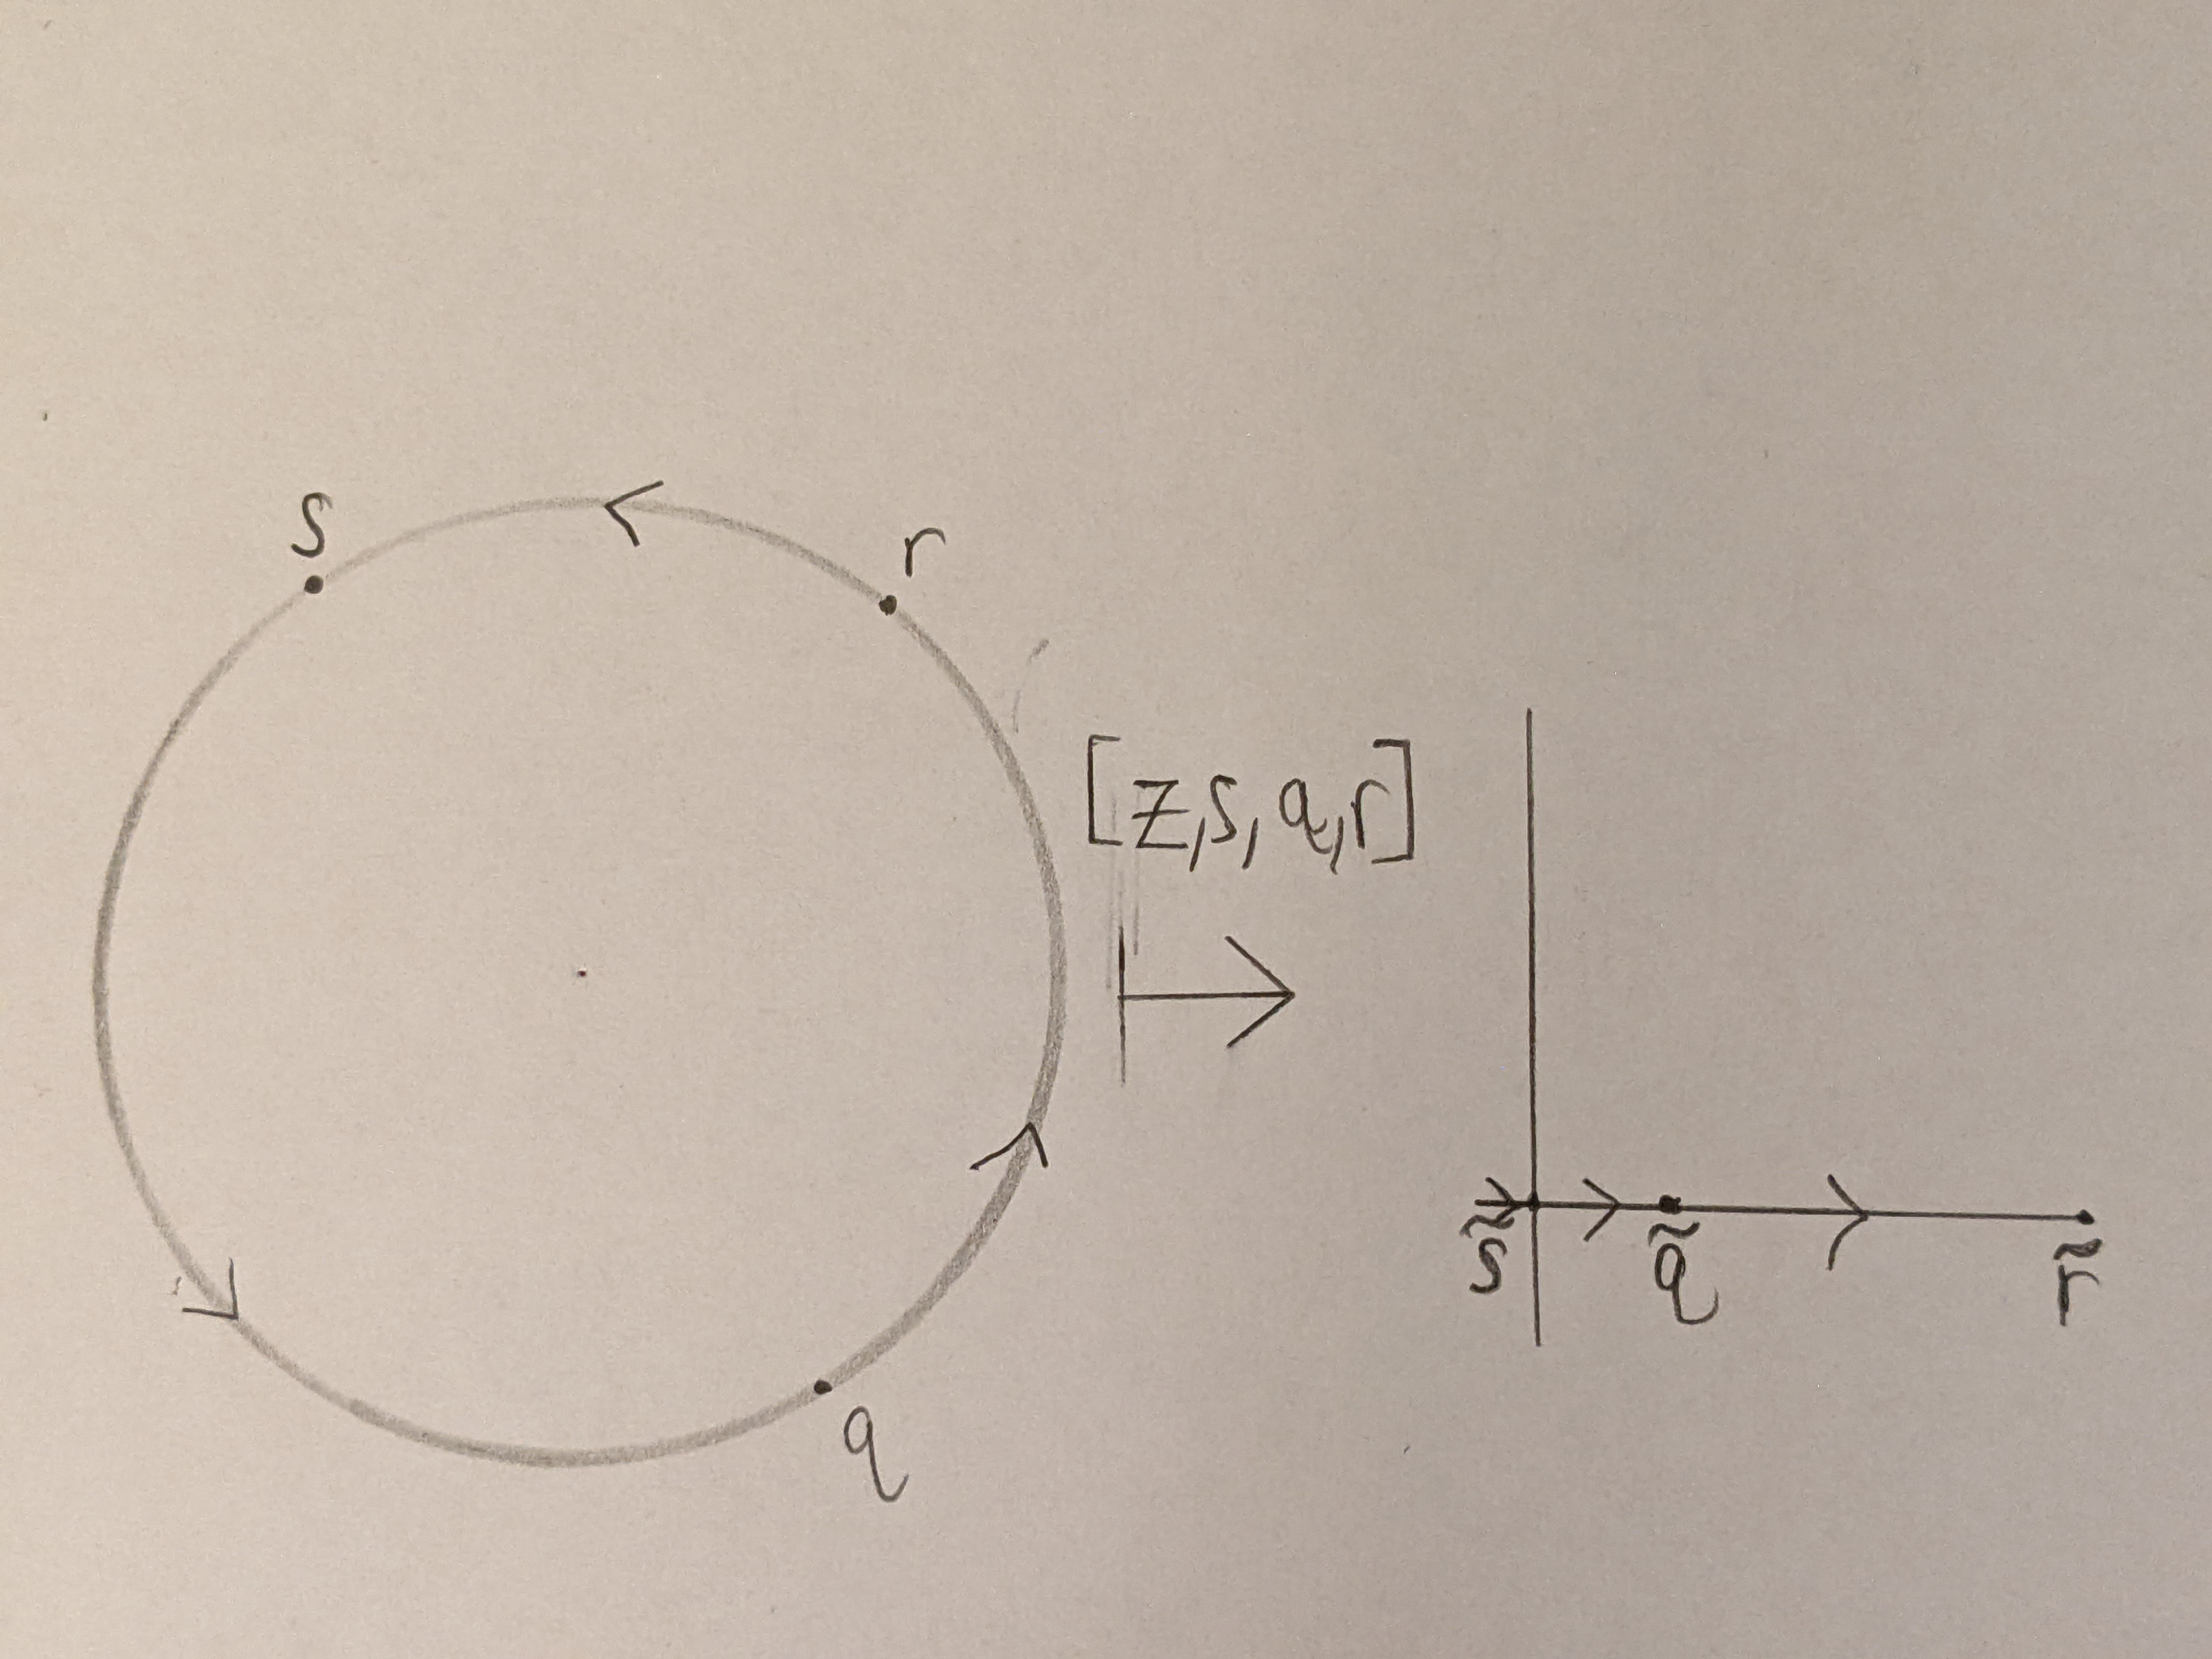
\includegraphics[width=\textwidth]{Problem16Image5}
\end{figure}
\noindent In this image, $q$ is sent to $\tilde{q} = 1$, $r$ is sent to $\tilde{r} = \infty$, and $s$ is sent to $\tilde{s} = 0$. Since $J \circ [z,q,r,s]$ and $[z,s,q,r]$ agree on the three points $q$, $r$, and $s$, we may deduce that $J \circ [z,q,r,s] = [z,s,q,r]$.
\subsection*{Part IV}
Notice that $\chi = [z,q,r,s]$, $I \circ \chi = I \circ [z,q,r,s] = [z,s,r,q]$, $J \circ \chi = J \circ [z,q,r,s] = [z,s,q,r]$, $I \circ J \circ \chi = I \circ [z,s,q,r] = [z,r,q,s]$, $J \circ I \circ \chi = J \circ [z,s,r,q] = [z,q,s,r]$, and $I \circ J \circ I \circ \chi = I \circ [z,q,s,r] = [z,r,s,q]$. Notice that these include all six permutations of the points $q$, $r$, and $s$, so they must include all six Mobius transformations in part $I$.
\subsection*{Part V}
The Mobius transformation $I$ fixes $1$ and swaps $0$ with $\infty$. Notice that $1/1 = 1$, $1/0 = \infty$, and $1/\infty = 0$. Since $I$ and $1/z$ agree on the points $0$, $1$, and $\infty$, we find that $I(z) = 1/z$. The Mobius transformation $J$ sends $0,1,\infty$ to $1,\infty,0$. Notice that $1/(1-0) = 1$, $1/(1-1) = 1/0 = \infty$, and $1/(1-\infty) = 0$. Since $J(z)$ and $1/(1-z)$ agree on the three points $0$, $1$, and $\infty$, we find that $J(z) = 1/(1-z)$.
\subsection*{Part VI}
As we noted in part iv, $\chi$, $I \circ \chi$, $J \circ \chi$, $I \circ J \circ \chi$, $J \circ I \circ \chi$, and $I \circ J \circ I \circ \chi$ represent all possible cross ratios. Using the fact that $I(z) = 1/z$ and $J(z) = 1/(1-z)$, we find that the cross ratios are
\[
\chi
\] and
\[
I \circ \chi = \frac{1}{\chi}
\] and
\[
J \circ \chi = \frac{1}{1-\chi}
\] and
\[
I \circ J \circ \chi = I\bigg( \frac{1}{1-\chi}\bigg) = 1-\chi
\] and
\[
J \circ I \circ \chi = J\bigg(\frac{1}{\chi}\bigg) = \frac{1}{1-\frac{1}{\chi}} = \frac{\chi}{\chi - 1}
\] and 
\[
I \circ J \circ I \circ \chi = I\bigg(\frac{\chi}{\chi - 1}\bigg) = \frac{\chi - 1}{\chi}
\]
\end{document} 